% =====================================================================
%  _ugnn_preamble.tex  --  SHARED preamble fragment for the U-GNN figures
%  (reference: oarfish-9)
%
%  \input this ONCE, in the PREAMBLE, from EITHER:
%    * the standalone wrapper  ugnn_architecture_full.tex  (local 2-page preview), OR
%    * your paper's main.tex   (to embed ugnn_fig1.tex / ugnn_fig2.tex).
%
%  Provides: TikZ libraries, the categorical colour palette, every math glyph
%  macro (\bb*, \Phi*, \Pi*, \Psi*, \theta*), and the caption toggle.  The glyph
%  macros use \providecommand, so if your paper ALREADY defines e.g. \bbS, your
%  definition wins and nothing clashes.
%
%  REQUIRES tikz + amsmath already loaded (tikz pulls in xcolor for \definecolor).
%
%  ---- paper-side usage -------------------------------------------------
%  preamble:
%     \usepackage{tikz}\usepackage{amsmath}\usepackage{graphicx}
%     % =====================================================================
%  _ugnn_preamble.tex  --  SHARED preamble fragment for the U-GNN figures
%  (reference: oarfish-9)
%
%  \input this ONCE, in the PREAMBLE, from EITHER:
%    * the standalone wrapper  ugnn_architecture_full.tex  (local 2-page preview), OR
%    * your paper's main.tex   (to embed ugnn_fig1.tex / ugnn_fig2.tex).
%
%  Provides: TikZ libraries, the categorical colour palette, every math glyph
%  macro (\bb*, \Phi*, \Pi*, \Psi*, \theta*), and the caption toggle.  The glyph
%  macros use \providecommand, so if your paper ALREADY defines e.g. \bbS, your
%  definition wins and nothing clashes.
%
%  REQUIRES tikz + amsmath already loaded (tikz pulls in xcolor for \definecolor).
%
%  ---- paper-side usage -------------------------------------------------
%  preamble:
%     \usepackage{tikz}\usepackage{amsmath}\usepackage{graphicx}
%     % =====================================================================
%  _ugnn_preamble.tex  --  SHARED preamble fragment for the U-GNN figures
%  (reference: oarfish-9)
%
%  \input this ONCE, in the PREAMBLE, from EITHER:
%    * the standalone wrapper  ugnn_architecture_full.tex  (local 2-page preview), OR
%    * your paper's main.tex   (to embed ugnn_fig1.tex / ugnn_fig2.tex).
%
%  Provides: TikZ libraries, the categorical colour palette, every math glyph
%  macro (\bb*, \Phi*, \Pi*, \Psi*, \theta*), and the caption toggle.  The glyph
%  macros use \providecommand, so if your paper ALREADY defines e.g. \bbS, your
%  definition wins and nothing clashes.
%
%  REQUIRES tikz + amsmath already loaded (tikz pulls in xcolor for \definecolor).
%
%  ---- paper-side usage -------------------------------------------------
%  preamble:
%     \usepackage{tikz}\usepackage{amsmath}\usepackage{graphicx}
%     % =====================================================================
%  _ugnn_preamble.tex  --  SHARED preamble fragment for the U-GNN figures
%  (reference: oarfish-9)
%
%  \input this ONCE, in the PREAMBLE, from EITHER:
%    * the standalone wrapper  ugnn_architecture_full.tex  (local 2-page preview), OR
%    * your paper's main.tex   (to embed ugnn_fig1.tex / ugnn_fig2.tex).
%
%  Provides: TikZ libraries, the categorical colour palette, every math glyph
%  macro (\bb*, \Phi*, \Pi*, \Psi*, \theta*), and the caption toggle.  The glyph
%  macros use \providecommand, so if your paper ALREADY defines e.g. \bbS, your
%  definition wins and nothing clashes.
%
%  REQUIRES tikz + amsmath already loaded (tikz pulls in xcolor for \definecolor).
%
%  ---- paper-side usage -------------------------------------------------
%  preamble:
%     \usepackage{tikz}\usepackage{amsmath}\usepackage{graphicx}
%     \input{path/to/_ugnn_preamble}
%     \showcaptionfalse            % paper supplies its own \caption{}
%  body:
%     \begin{figure*}[t]\centering
%       \resizebox{\textwidth}{!}{\input{path/to/ugnn_fig1}}
%       \caption{...}\label{fig:ugnn}
%     \end{figure*}
%     \begin{figure*}[t]\centering
%       \resizebox{\textwidth}{!}{\input{path/to/ugnn_fig2}}
%       \caption{...}\label{fig:ugnn-block}
%     \end{figure*}
%  NB embedded, fonts inherit YOUR paper's class (not extarticle 17pt);
%  \resizebox scales the whole picture, so it stays internally consistent.
% =====================================================================
\usetikzlibrary{arrows.meta, positioning, calc, backgrounds, fit}

% ===== categorical block palette =====================================
%   green  = GNN  (phi^enc / phi^dec / phi^bn)
%   purple = projection layers (Pi_0, Pi^cond, Pi^step, Pi_b, Pi^skip, Pi_out)
%   orange = learned node selector (Psi_b)  -- matches its C_b control edges
%   red / blue are RESERVED for the encoder / decoder panels.
\definecolor{gnncol}{RGB}{200,230,190}
\definecolor{projcol}{RGB}{223,201,234}
\definecolor{selcol}{RGB}{250,205,158}
\definecolor{bandcol}{RGB}{176,130,80}   % depth-band base (warm golden sand; swap freely)

% ===== math glyphs (\providecommand: figure owns them, but a paper that ====
% ===== already defines the symbol keeps its own version, no clash) ========
\providecommand{\bbS}{\mathbf{S}}
\providecommand{\bbC}{\mathbf{C}}
\providecommand{\bbD}{\mathbf{D}}
\providecommand{\bbZ}{\mathbf{Z}}
\providecommand{\bbY}{\mathbf{Y}}
\providecommand{\bbU}{\mathbf{U}}
\providecommand{\bbK}{\mathbf{K}}
\providecommand{\bbP}{\mathbf{P}}
\providecommand{\bbV}{\mathbf{V}}
\providecommand{\bbI}{\mathbf{I}}
\providecommand{\bbvv}{\mathbf{v}}
\providecommand{\bbx}{\mathbf{x}}
\providecommand{\bbu}{\mathbf{u}}
\providecommand{\bbeps}{\boldsymbol{\epsilon}_{\boldsymbol{\theta}}}
\providecommand{\bbepsilon}{\boldsymbol{\epsilon}}      % bare epsilon (subscript supplied at use site)
\providecommand{\bbtheta}{\boldsymbol{\theta}}
\providecommand{\bbxi}{\boldsymbol{\xi}}                % compact conditioning placeholder (S,u,...)
\providecommand{\alphacumprod}{\bar{\alpha}}            % cumulative-product noise schedule constant
\providecommand{\UK}{[\bbU_0;\bbK_0]}
% GNN operators (single symbol phi, role superscript)
\providecommand{\PhiEnc}[1]{\boldsymbol{\Phi}^{\mathrm{E}}_{#1}}
\providecommand{\PhiDec}[1]{\boldsymbol{\Phi}^{\mathrm{D}}_{#1}}
\providecommand{\PhiBn}{\boldsymbol{\Phi}^{\mathrm{B}}}
% projection / embedding family
\providecommand{\Piin}{\Pi_{0}}
\providecommand{\Picond}{\Pi^{\mathrm{cond}}_{0}}
\providecommand{\Pistep}{\Pi^{\mathrm{step}}_{0}}
\providecommand{\Piblk}[1]{\Pi_{#1}}
\providecommand{\Piskip}[1]{\Pi^{\mathrm{skip}}_{#1}}
\providecommand{\Piout}{\Pi_{\mathrm{out}}}
% scoring head
\providecommand{\Psisel}[1]{\boldsymbol{\Psi}_{#1}}
% learnable parameters
\providecommand{\thetaenc}{\boldsymbol{\Theta}^{\mathrm{E}}}
\providecommand{\thetadec}{\boldsymbol{\Theta}^{\mathrm{D}}}
\providecommand{\thetasel}{\boldsymbol{\Theta}^{\mathrm{sel}}}

% ===== caption toggle (build option) =================================
% Captions ON by default.  Turn OFF either way:
%   * after this \input:  \showcaptionfalse        (e.g. when embedding in a paper)
%   * on the command line: pdflatex "\def\nocaption{}\input{ugnn_architecture_full}"
% Guarded so a double \input cannot redefine/reset the flag.
\ifdefined\ifshowcaption\else \newif\ifshowcaption \showcaptiontrue \fi
\ifdefined\nocaption\showcaptionfalse\fi

%     \showcaptionfalse            % paper supplies its own \caption{}
%  body:
%     \begin{figure*}[t]\centering
%       \resizebox{\textwidth}{!}{\input{path/to/ugnn_fig1}}
%       \caption{...}\label{fig:ugnn}
%     \end{figure*}
%     \begin{figure*}[t]\centering
%       \resizebox{\textwidth}{!}{% ugnn_fig2.tex -- Fig 2 body (block-interface inset). Drawing only.
% \input AFTER _ugnn_preamble.tex.
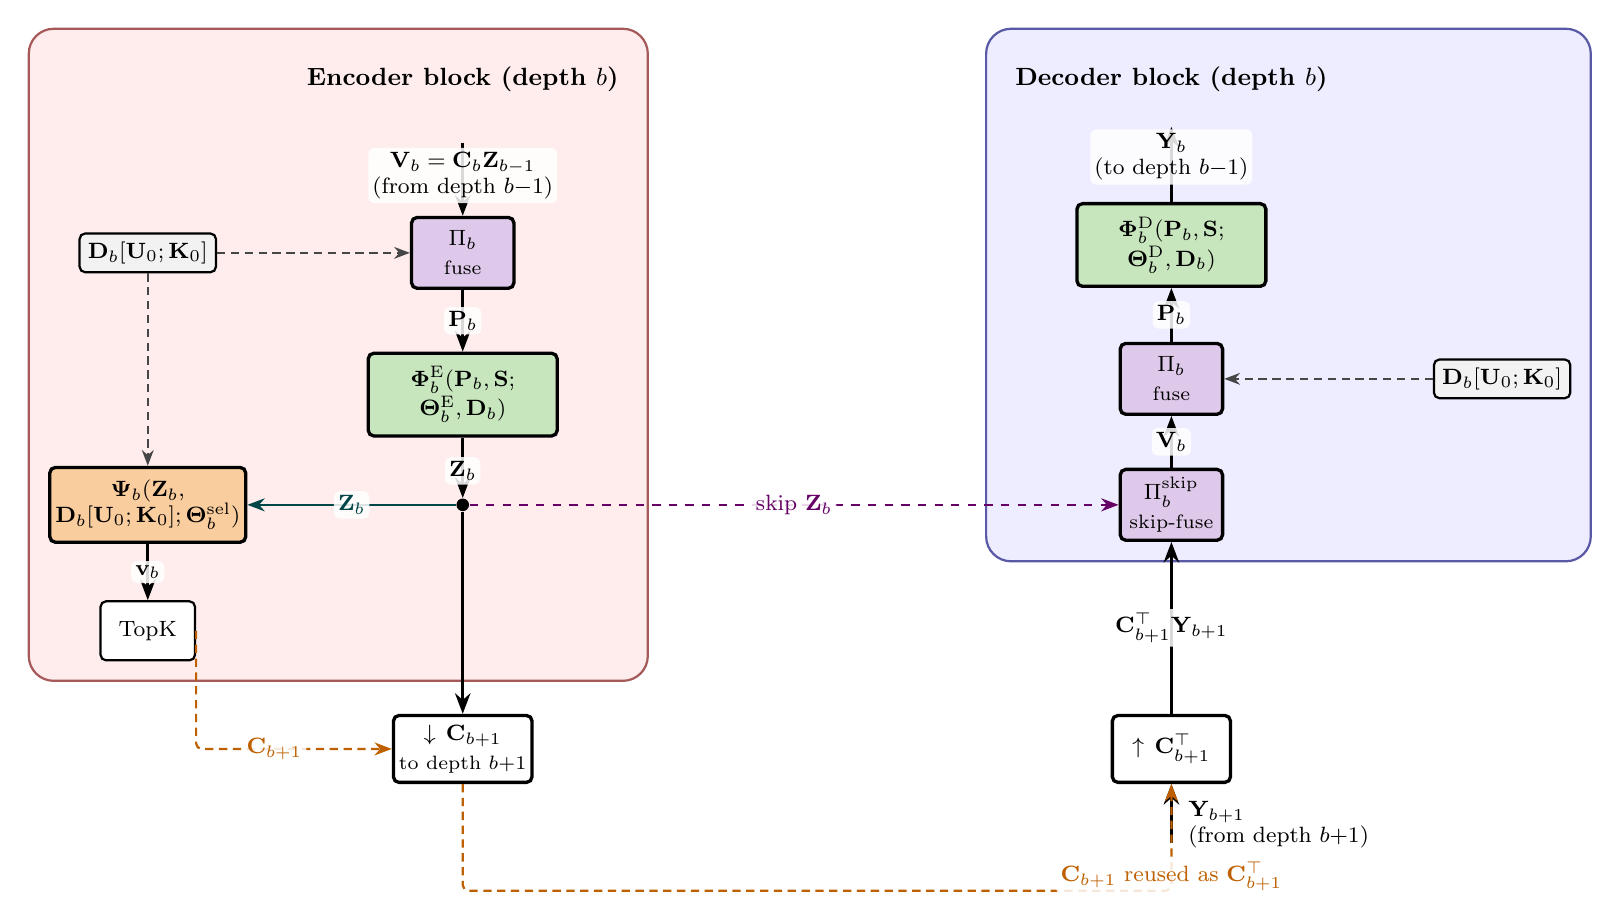
\begin{tikzpicture}[
  >={Stealth[length=2.6mm]},
  rounded corners=2pt,
  proc/.style    = {draw, very thick, rounded corners=2pt, align=center,
                    minimum width=2.4cm, minimum height=1.05cm, inner sep=2pt,
                    font=\footnotesize, fill=gnncol},   % GNN green
  fuseb/.style   = {draw, very thick, rounded corners=2pt, align=center,
                    minimum width=1.3cm, minimum height=0.9cm, inner sep=2pt,
                    font=\footnotesize, fill=projcol},  % projection amber
  encbg/.style   = {rounded corners=9pt, fill=red!7,  draw=red!30!gray, thick,
                    inner sep=7pt},
  decbg/.style   = {rounded corners=9pt, fill=blue!7, draw=blue!30!gray, thick,
                    inner sep=7pt},
  selb/.style    = {draw, very thick, rounded corners=2pt, align=center,
                    minimum width=2.4cm, minimum height=0.95cm, inner sep=2pt,
                    font=\footnotesize, fill=selcol},
  sampb/.style   = {draw, very thick, rounded corners=2pt, align=center,
                    minimum width=1.5cm, minimum height=0.85cm, inner sep=2pt,
                    font=\footnotesize, fill=white},
  condb/.style   = {draw, thick, rounded corners=2pt, align=center,
                    inner sep=3pt, font=\footnotesize, fill=black!5},
  topkb/.style   = {draw, thick, rounded corners=2pt, align=center,
                    minimum width=1.2cm, minimum height=0.75cm, inner sep=2pt,
                    font=\footnotesize, fill=white},
  splitdot/.style= {circle, fill=black, inner sep=0pt, minimum size=1.6mm},
  sig/.style     = {-{Stealth[length=2.6mm]}, very thick},
  feat/.style    = {-{Stealth[length=2.2mm]}, thick, teal!55!black},
  ctrl/.style    = {-{Stealth[length=2.2mm]}, thick, densely dashed, orange!75!black},
  skip/.style    = {-{Stealth[length=2.2mm]}, thick, dashed, violet!80!black},
  condarr/.style = {-{Stealth[length=2.0mm]}, thick, gray!55!black, densely dashed},
  elbl/.style    = {font=\footnotesize, inner sep=1.5pt, fill=white,
                    fill opacity=0.85, text opacity=1},
  hd/.style      = {font=\small\bfseries},
]

% ---------- ENCODER block (depth b) : flows top -> down ----------
\node[fuseb] (Epi)   at (0,6.8) {$\Piblk{b}$\\[1pt]{\scriptsize fuse}};
\node[proc]  (Egnn)  at (0,5.0) {$\PhiEnc{b}(\bbP_b,\bbS;$\\$\thetaenc_b,\bbD_b)$};
\node[splitdot](Esp) at (0,3.6) {};
\node[sampb] (Edown) at (0,0.5) {$\downarrow\,\bbC_{b+1}$\\[1pt]{\scriptsize to depth $b{+}1$}};  % OUTSIDE panel
\node[condb] (Econd) at (-4.0,6.8) {$\bbD_b\UK$};
\node[selb]  (Epsi)  at (-4.0,3.6) {$\Psisel{b}(\bbZ_b,$\\$\bbD_b\UK;\thetasel_{b})$};
\node[topkb] (Etopk) at (-4.0,2.0) {$\mathrm{TopK}$};

\draw[sig]  (0,8.2) -- (Epi.north)
            node[elbl,pos=0.45,align=center]{$\bbV_b=\bbC_b\bbZ_{b-1}$\\(from depth $b{-}1$)};
\draw[condarr] (Econd.east) -- (Epi.west);
\draw[sig]  (Epi.south)  -- (Egnn.north) node[elbl,pos=0.5]{$\bbP_b$};
\draw[sig]  (Egnn.south) -- (Esp)        node[elbl,pos=0.55]{$\bbZ_b$};
\draw[sig]  (Esp) -- (Edown.north);
\draw[feat] (Esp) -- (Epsi.east)         node[elbl,pos=0.5]{$\bbZ_b$};
\draw[condarr] (Econd.south) -- (Epsi.north);
\draw[sig]  (Epsi.south) -- (Etopk.north) node[elbl,pos=0.5]{$\bbvv_{b}$};
\draw[ctrl] (Etopk.east) |- (Edown.west)  node[elbl,pos=0.7]{$\bbC_{b+1}$};

% ---------- DECODER block (depth b) : flows bottom -> up ----------
\node[sampb] (Dup)   at (9,0.5) {$\uparrow\,\bbC_{b+1}^{\top}$};  % OUTSIDE panel
\node[fuseb] (Dskip) at (9,3.6) {$\Piskip{b}$\\[1pt]{\scriptsize skip-fuse}};
\node[fuseb] (Dpi)   at (9,5.2) {$\Piblk{b}$\\[1pt]{\scriptsize fuse}};
\node[proc]  (Dgnn)  at (9,6.9) {$\PhiDec{b}(\bbP_b,\bbS;$\\$\thetadec_b,\bbD_b)$};
\node[condb] (Dcond) at (13.2,5.2) {$\bbD_b\UK$};

\draw[sig]  (9,-0.7) -- (Dup.south)
            node[elbl,pos=0.32,align=left,anchor=west,xshift=4pt]{$\bbY_{b+1}$\\(from depth $b{+}1$)};
\draw[sig]  (Dup.north)   -- (Dskip.south) node[elbl,pos=0.5]{$\bbC_{b+1}^{\top}\bbY_{b+1}$};
\draw[sig]  (Dskip.north) -- (Dpi.south)   node[elbl,pos=0.5]{$\bbV_b$};
\draw[condarr] (Dcond.west) -- (Dpi.east);
\draw[sig]  (Dpi.north)   -- (Dgnn.south)  node[elbl,pos=0.5]{$\bbP_b$};
\draw[sig]  (Dgnn.north)  -- (9,8.4)
            node[elbl,pos=0.6,align=center]{$\bbY_b$\\(to depth $b{-}1$)};

% ---------- cross-links between the two blocks ----------
% skip Z_b : encoder split -> decoder skip-fusion
\draw[skip] (Esp) -- (Dskip.west) node[elbl,pos=0.5]{skip $\bbZ_b$};
% reuse C_{b+1} : encoder selector -> decoder up-sampling
\draw[ctrl] (Edown.south) -- (0,-1.3) -- (9,-1.3) -- (Dup.south)
            node[elbl,pos=0.32,below]{$\bbC_{b+1}$ reused as $\bbC_{b+1}^{\top}$};

% ---------- headers + caption ----------
\node[hd] (Ehdr) at (0,9.0)  {Encoder block (depth $b$)};
\node[hd] (Dhdr) at (9,9.0)  {Decoder block (depth $b$)};

% ---------- half-panel background tints (light red / light blue) ----------
\begin{scope}[on background layer]
  \node[encbg, fit={(Ehdr)(Econd)(Epi)(Egnn)(Esp)(Epsi)(Etopk)(0,9.4)}] {};
  \node[decbg, fit={(Dhdr)(Dskip)(Dpi)(Dgnn)(Dcond)(9,9.4)}] {};
\end{scope}

\ifshowcaption
\node[font=\small, align=center] at (4.5,-2.3)
  {\textbf{Fig.~2.} Block interface. The fusion layer $\Piblk{b}$ is shared across the
   matched encoder/decoder pair; the selection matrix $\bbC_{b+1}$ produced by
   $\Psisel{b}$ on the encoder side is reused (transposed) by the decoder's
   up-sampling. Global embeddings enter as $\bbD_b\UK$.};
\fi

\end{tikzpicture}
}
%       \caption{...}\label{fig:ugnn-block}
%     \end{figure*}
%  NB embedded, fonts inherit YOUR paper's class (not extarticle 17pt);
%  \resizebox scales the whole picture, so it stays internally consistent.
% =====================================================================
\usetikzlibrary{arrows.meta, positioning, calc, backgrounds, fit}

% ===== categorical block palette =====================================
%   green  = GNN  (phi^enc / phi^dec / phi^bn)
%   purple = projection layers (Pi_0, Pi^cond, Pi^step, Pi_b, Pi^skip, Pi_out)
%   orange = learned node selector (Psi_b)  -- matches its C_b control edges
%   red / blue are RESERVED for the encoder / decoder panels.
\definecolor{gnncol}{RGB}{200,230,190}
\definecolor{projcol}{RGB}{223,201,234}
\definecolor{selcol}{RGB}{250,205,158}
\definecolor{bandcol}{RGB}{176,130,80}   % depth-band base (warm golden sand; swap freely)

% ===== math glyphs (\providecommand: figure owns them, but a paper that ====
% ===== already defines the symbol keeps its own version, no clash) ========
\providecommand{\bbS}{\mathbf{S}}
\providecommand{\bbC}{\mathbf{C}}
\providecommand{\bbD}{\mathbf{D}}
\providecommand{\bbZ}{\mathbf{Z}}
\providecommand{\bbY}{\mathbf{Y}}
\providecommand{\bbU}{\mathbf{U}}
\providecommand{\bbK}{\mathbf{K}}
\providecommand{\bbP}{\mathbf{P}}
\providecommand{\bbV}{\mathbf{V}}
\providecommand{\bbI}{\mathbf{I}}
\providecommand{\bbvv}{\mathbf{v}}
\providecommand{\bbx}{\mathbf{x}}
\providecommand{\bbu}{\mathbf{u}}
\providecommand{\bbeps}{\boldsymbol{\epsilon}_{\boldsymbol{\theta}}}
\providecommand{\bbepsilon}{\boldsymbol{\epsilon}}      % bare epsilon (subscript supplied at use site)
\providecommand{\bbtheta}{\boldsymbol{\theta}}
\providecommand{\bbxi}{\boldsymbol{\xi}}                % compact conditioning placeholder (S,u,...)
\providecommand{\alphacumprod}{\bar{\alpha}}            % cumulative-product noise schedule constant
\providecommand{\UK}{[\bbU_0;\bbK_0]}
% GNN operators (single symbol phi, role superscript)
\providecommand{\PhiEnc}[1]{\boldsymbol{\Phi}^{\mathrm{E}}_{#1}}
\providecommand{\PhiDec}[1]{\boldsymbol{\Phi}^{\mathrm{D}}_{#1}}
\providecommand{\PhiBn}{\boldsymbol{\Phi}^{\mathrm{B}}}
% projection / embedding family
\providecommand{\Piin}{\Pi_{0}}
\providecommand{\Picond}{\Pi^{\mathrm{cond}}_{0}}
\providecommand{\Pistep}{\Pi^{\mathrm{step}}_{0}}
\providecommand{\Piblk}[1]{\Pi_{#1}}
\providecommand{\Piskip}[1]{\Pi^{\mathrm{skip}}_{#1}}
\providecommand{\Piout}{\Pi_{\mathrm{out}}}
% scoring head
\providecommand{\Psisel}[1]{\boldsymbol{\Psi}_{#1}}
% learnable parameters
\providecommand{\thetaenc}{\boldsymbol{\Theta}^{\mathrm{E}}}
\providecommand{\thetadec}{\boldsymbol{\Theta}^{\mathrm{D}}}
\providecommand{\thetasel}{\boldsymbol{\Theta}^{\mathrm{sel}}}

% ===== caption toggle (build option) =================================
% Captions ON by default.  Turn OFF either way:
%   * after this \input:  \showcaptionfalse        (e.g. when embedding in a paper)
%   * on the command line: pdflatex "\def\nocaption{}% =====================================================================
%  U-GNN denoiser architecture  (reference: oarfish-9)  --  STANDALONE WRAPPER
%
%  This file is now a THIN WRAPPER, used only for local 2-page preview.
%  The actual drawing code lives in three sibling files:
%      _ugnn_preamble.tex  -- shared colours, glyph macros, caption toggle
%      ugnn_fig1.tex       -- Fig 1 (high-level encoder-decoder U)
%      ugnn_fig2.tex       -- Fig 2 (block-interface inset)
%  To EMBED the figures in a paper, \input the preamble + each body file
%  directly into your main.tex (see the header of _ugnn_preamble.tex for the
%  exact snippet); do NOT \input this wrapper.
%
%  Notation (single GNN symbol phi; conditioning fused by Pi_b before phi):
%    encoder    Z_b   = Phi^E_b ( P_b , S ; Theta^enc_b , D_b )
%    decoder    Y_b   = Phi^D_b ( P_b , S ; Theta^dec_b , D_b )
%    bottleneck Y_{B+1}= Phi^B  ( C_{B+1} Z_B , S ; Theta^bn , D_{B+1} )
%    block fuse P_b   = Pi_b ( V_b , D_b [U_0;K_0] )
%    selection (depth-b selector)  v_b = Psi_b ( Z_b , D_b[U_0;K_0] ) ; C_{b+1} = TopK(v_b)
%
%  Compile (with captions):  pdflatex ugnn_architecture_full.tex
%  Compile (no captions):    pdflatex "\def\nocaption{}\input{ugnn_architecture_full}"
% =====================================================================
\documentclass[tikz,border=12pt,class=extarticle,17pt]{standalone}   % extarticle 17pt base: bigger global fonts
\usepackage{amsmath}
\input{_ugnn_preamble}

\begin{document}
\input{ugnn_fig1}
\newpage
\input{ugnn_fig2}
\end{document}
"
% Guarded so a double \input cannot redefine/reset the flag.
\ifdefined\ifshowcaption\else \newif\ifshowcaption \showcaptiontrue \fi
\ifdefined\nocaption\showcaptionfalse\fi

%     \showcaptionfalse            % paper supplies its own \caption{}
%  body:
%     \begin{figure*}[t]\centering
%       \resizebox{\textwidth}{!}{\input{path/to/ugnn_fig1}}
%       \caption{...}\label{fig:ugnn}
%     \end{figure*}
%     \begin{figure*}[t]\centering
%       \resizebox{\textwidth}{!}{% ugnn_fig2.tex -- Fig 2 body (block-interface inset). Drawing only.
% \input AFTER _ugnn_preamble.tex.
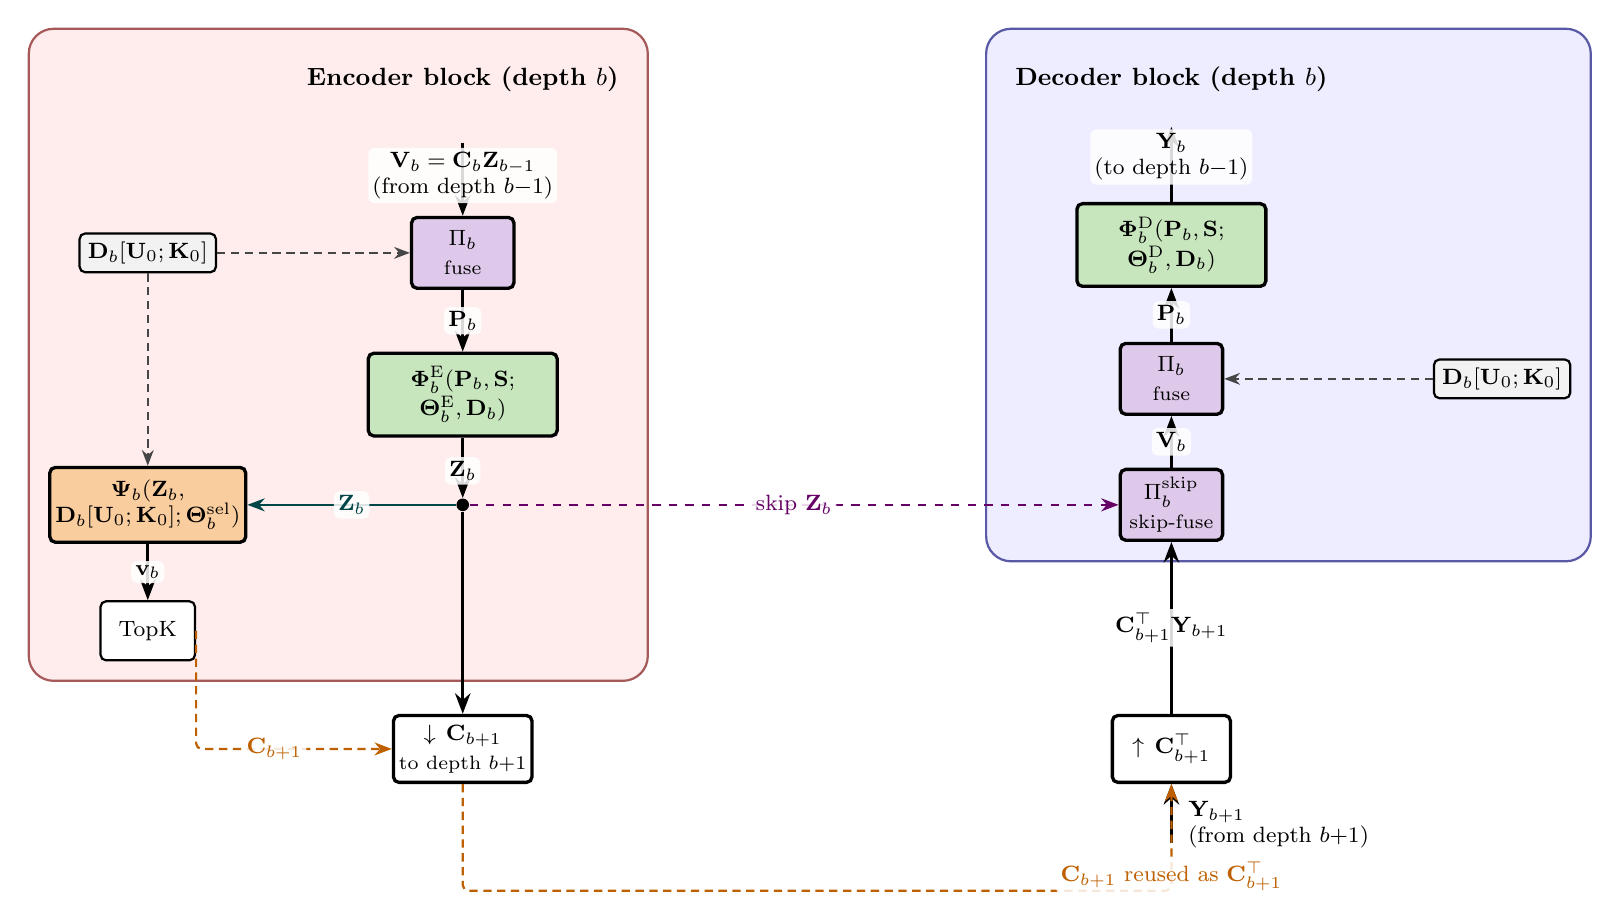
\begin{tikzpicture}[
  >={Stealth[length=2.6mm]},
  rounded corners=2pt,
  proc/.style    = {draw, very thick, rounded corners=2pt, align=center,
                    minimum width=2.4cm, minimum height=1.05cm, inner sep=2pt,
                    font=\footnotesize, fill=gnncol},   % GNN green
  fuseb/.style   = {draw, very thick, rounded corners=2pt, align=center,
                    minimum width=1.3cm, minimum height=0.9cm, inner sep=2pt,
                    font=\footnotesize, fill=projcol},  % projection amber
  encbg/.style   = {rounded corners=9pt, fill=red!7,  draw=red!30!gray, thick,
                    inner sep=7pt},
  decbg/.style   = {rounded corners=9pt, fill=blue!7, draw=blue!30!gray, thick,
                    inner sep=7pt},
  selb/.style    = {draw, very thick, rounded corners=2pt, align=center,
                    minimum width=2.4cm, minimum height=0.95cm, inner sep=2pt,
                    font=\footnotesize, fill=selcol},
  sampb/.style   = {draw, very thick, rounded corners=2pt, align=center,
                    minimum width=1.5cm, minimum height=0.85cm, inner sep=2pt,
                    font=\footnotesize, fill=white},
  condb/.style   = {draw, thick, rounded corners=2pt, align=center,
                    inner sep=3pt, font=\footnotesize, fill=black!5},
  topkb/.style   = {draw, thick, rounded corners=2pt, align=center,
                    minimum width=1.2cm, minimum height=0.75cm, inner sep=2pt,
                    font=\footnotesize, fill=white},
  splitdot/.style= {circle, fill=black, inner sep=0pt, minimum size=1.6mm},
  sig/.style     = {-{Stealth[length=2.6mm]}, very thick},
  feat/.style    = {-{Stealth[length=2.2mm]}, thick, teal!55!black},
  ctrl/.style    = {-{Stealth[length=2.2mm]}, thick, densely dashed, orange!75!black},
  skip/.style    = {-{Stealth[length=2.2mm]}, thick, dashed, violet!80!black},
  condarr/.style = {-{Stealth[length=2.0mm]}, thick, gray!55!black, densely dashed},
  elbl/.style    = {font=\footnotesize, inner sep=1.5pt, fill=white,
                    fill opacity=0.85, text opacity=1},
  hd/.style      = {font=\small\bfseries},
]

% ---------- ENCODER block (depth b) : flows top -> down ----------
\node[fuseb] (Epi)   at (0,6.8) {$\Piblk{b}$\\[1pt]{\scriptsize fuse}};
\node[proc]  (Egnn)  at (0,5.0) {$\PhiEnc{b}(\bbP_b,\bbS;$\\$\thetaenc_b,\bbD_b)$};
\node[splitdot](Esp) at (0,3.6) {};
\node[sampb] (Edown) at (0,0.5) {$\downarrow\,\bbC_{b+1}$\\[1pt]{\scriptsize to depth $b{+}1$}};  % OUTSIDE panel
\node[condb] (Econd) at (-4.0,6.8) {$\bbD_b\UK$};
\node[selb]  (Epsi)  at (-4.0,3.6) {$\Psisel{b}(\bbZ_b,$\\$\bbD_b\UK;\thetasel_{b})$};
\node[topkb] (Etopk) at (-4.0,2.0) {$\mathrm{TopK}$};

\draw[sig]  (0,8.2) -- (Epi.north)
            node[elbl,pos=0.45,align=center]{$\bbV_b=\bbC_b\bbZ_{b-1}$\\(from depth $b{-}1$)};
\draw[condarr] (Econd.east) -- (Epi.west);
\draw[sig]  (Epi.south)  -- (Egnn.north) node[elbl,pos=0.5]{$\bbP_b$};
\draw[sig]  (Egnn.south) -- (Esp)        node[elbl,pos=0.55]{$\bbZ_b$};
\draw[sig]  (Esp) -- (Edown.north);
\draw[feat] (Esp) -- (Epsi.east)         node[elbl,pos=0.5]{$\bbZ_b$};
\draw[condarr] (Econd.south) -- (Epsi.north);
\draw[sig]  (Epsi.south) -- (Etopk.north) node[elbl,pos=0.5]{$\bbvv_{b}$};
\draw[ctrl] (Etopk.east) |- (Edown.west)  node[elbl,pos=0.7]{$\bbC_{b+1}$};

% ---------- DECODER block (depth b) : flows bottom -> up ----------
\node[sampb] (Dup)   at (9,0.5) {$\uparrow\,\bbC_{b+1}^{\top}$};  % OUTSIDE panel
\node[fuseb] (Dskip) at (9,3.6) {$\Piskip{b}$\\[1pt]{\scriptsize skip-fuse}};
\node[fuseb] (Dpi)   at (9,5.2) {$\Piblk{b}$\\[1pt]{\scriptsize fuse}};
\node[proc]  (Dgnn)  at (9,6.9) {$\PhiDec{b}(\bbP_b,\bbS;$\\$\thetadec_b,\bbD_b)$};
\node[condb] (Dcond) at (13.2,5.2) {$\bbD_b\UK$};

\draw[sig]  (9,-0.7) -- (Dup.south)
            node[elbl,pos=0.32,align=left,anchor=west,xshift=4pt]{$\bbY_{b+1}$\\(from depth $b{+}1$)};
\draw[sig]  (Dup.north)   -- (Dskip.south) node[elbl,pos=0.5]{$\bbC_{b+1}^{\top}\bbY_{b+1}$};
\draw[sig]  (Dskip.north) -- (Dpi.south)   node[elbl,pos=0.5]{$\bbV_b$};
\draw[condarr] (Dcond.west) -- (Dpi.east);
\draw[sig]  (Dpi.north)   -- (Dgnn.south)  node[elbl,pos=0.5]{$\bbP_b$};
\draw[sig]  (Dgnn.north)  -- (9,8.4)
            node[elbl,pos=0.6,align=center]{$\bbY_b$\\(to depth $b{-}1$)};

% ---------- cross-links between the two blocks ----------
% skip Z_b : encoder split -> decoder skip-fusion
\draw[skip] (Esp) -- (Dskip.west) node[elbl,pos=0.5]{skip $\bbZ_b$};
% reuse C_{b+1} : encoder selector -> decoder up-sampling
\draw[ctrl] (Edown.south) -- (0,-1.3) -- (9,-1.3) -- (Dup.south)
            node[elbl,pos=0.32,below]{$\bbC_{b+1}$ reused as $\bbC_{b+1}^{\top}$};

% ---------- headers + caption ----------
\node[hd] (Ehdr) at (0,9.0)  {Encoder block (depth $b$)};
\node[hd] (Dhdr) at (9,9.0)  {Decoder block (depth $b$)};

% ---------- half-panel background tints (light red / light blue) ----------
\begin{scope}[on background layer]
  \node[encbg, fit={(Ehdr)(Econd)(Epi)(Egnn)(Esp)(Epsi)(Etopk)(0,9.4)}] {};
  \node[decbg, fit={(Dhdr)(Dskip)(Dpi)(Dgnn)(Dcond)(9,9.4)}] {};
\end{scope}

\ifshowcaption
\node[font=\small, align=center] at (4.5,-2.3)
  {\textbf{Fig.~2.} Block interface. The fusion layer $\Piblk{b}$ is shared across the
   matched encoder/decoder pair; the selection matrix $\bbC_{b+1}$ produced by
   $\Psisel{b}$ on the encoder side is reused (transposed) by the decoder's
   up-sampling. Global embeddings enter as $\bbD_b\UK$.};
\fi

\end{tikzpicture}
}
%       \caption{...}\label{fig:ugnn-block}
%     \end{figure*}
%  NB embedded, fonts inherit YOUR paper's class (not extarticle 17pt);
%  \resizebox scales the whole picture, so it stays internally consistent.
% =====================================================================
\usetikzlibrary{arrows.meta, positioning, calc, backgrounds, fit}

% ===== categorical block palette =====================================
%   green  = GNN  (phi^enc / phi^dec / phi^bn)
%   purple = projection layers (Pi_0, Pi^cond, Pi^step, Pi_b, Pi^skip, Pi_out)
%   orange = learned node selector (Psi_b)  -- matches its C_b control edges
%   red / blue are RESERVED for the encoder / decoder panels.
\definecolor{gnncol}{RGB}{200,230,190}
\definecolor{projcol}{RGB}{223,201,234}
\definecolor{selcol}{RGB}{250,205,158}
\definecolor{bandcol}{RGB}{176,130,80}   % depth-band base (warm golden sand; swap freely)

% ===== math glyphs (\providecommand: figure owns them, but a paper that ====
% ===== already defines the symbol keeps its own version, no clash) ========
\providecommand{\bbS}{\mathbf{S}}
\providecommand{\bbC}{\mathbf{C}}
\providecommand{\bbD}{\mathbf{D}}
\providecommand{\bbZ}{\mathbf{Z}}
\providecommand{\bbY}{\mathbf{Y}}
\providecommand{\bbU}{\mathbf{U}}
\providecommand{\bbK}{\mathbf{K}}
\providecommand{\bbP}{\mathbf{P}}
\providecommand{\bbV}{\mathbf{V}}
\providecommand{\bbI}{\mathbf{I}}
\providecommand{\bbvv}{\mathbf{v}}
\providecommand{\bbx}{\mathbf{x}}
\providecommand{\bbu}{\mathbf{u}}
\providecommand{\bbeps}{\boldsymbol{\epsilon}_{\boldsymbol{\theta}}}
\providecommand{\bbepsilon}{\boldsymbol{\epsilon}}      % bare epsilon (subscript supplied at use site)
\providecommand{\bbtheta}{\boldsymbol{\theta}}
\providecommand{\bbxi}{\boldsymbol{\xi}}                % compact conditioning placeholder (S,u,...)
\providecommand{\alphacumprod}{\bar{\alpha}}            % cumulative-product noise schedule constant
\providecommand{\UK}{[\bbU_0;\bbK_0]}
% GNN operators (single symbol phi, role superscript)
\providecommand{\PhiEnc}[1]{\boldsymbol{\Phi}^{\mathrm{E}}_{#1}}
\providecommand{\PhiDec}[1]{\boldsymbol{\Phi}^{\mathrm{D}}_{#1}}
\providecommand{\PhiBn}{\boldsymbol{\Phi}^{\mathrm{B}}}
% projection / embedding family
\providecommand{\Piin}{\Pi_{0}}
\providecommand{\Picond}{\Pi^{\mathrm{cond}}_{0}}
\providecommand{\Pistep}{\Pi^{\mathrm{step}}_{0}}
\providecommand{\Piblk}[1]{\Pi_{#1}}
\providecommand{\Piskip}[1]{\Pi^{\mathrm{skip}}_{#1}}
\providecommand{\Piout}{\Pi_{\mathrm{out}}}
% scoring head
\providecommand{\Psisel}[1]{\boldsymbol{\Psi}_{#1}}
% learnable parameters
\providecommand{\thetaenc}{\boldsymbol{\Theta}^{\mathrm{E}}}
\providecommand{\thetadec}{\boldsymbol{\Theta}^{\mathrm{D}}}
\providecommand{\thetasel}{\boldsymbol{\Theta}^{\mathrm{sel}}}

% ===== caption toggle (build option) =================================
% Captions ON by default.  Turn OFF either way:
%   * after this \input:  \showcaptionfalse        (e.g. when embedding in a paper)
%   * on the command line: pdflatex "\def\nocaption{}% =====================================================================
%  U-GNN denoiser architecture  (reference: oarfish-9)  --  STANDALONE WRAPPER
%
%  This file is now a THIN WRAPPER, used only for local 2-page preview.
%  The actual drawing code lives in three sibling files:
%      _ugnn_preamble.tex  -- shared colours, glyph macros, caption toggle
%      ugnn_fig1.tex       -- Fig 1 (high-level encoder-decoder U)
%      ugnn_fig2.tex       -- Fig 2 (block-interface inset)
%  To EMBED the figures in a paper, \input the preamble + each body file
%  directly into your main.tex (see the header of _ugnn_preamble.tex for the
%  exact snippet); do NOT \input this wrapper.
%
%  Notation (single GNN symbol phi; conditioning fused by Pi_b before phi):
%    encoder    Z_b   = Phi^E_b ( P_b , S ; Theta^enc_b , D_b )
%    decoder    Y_b   = Phi^D_b ( P_b , S ; Theta^dec_b , D_b )
%    bottleneck Y_{B+1}= Phi^B  ( C_{B+1} Z_B , S ; Theta^bn , D_{B+1} )
%    block fuse P_b   = Pi_b ( V_b , D_b [U_0;K_0] )
%    selection (depth-b selector)  v_b = Psi_b ( Z_b , D_b[U_0;K_0] ) ; C_{b+1} = TopK(v_b)
%
%  Compile (with captions):  pdflatex ugnn_architecture_full.tex
%  Compile (no captions):    pdflatex "\def\nocaption{}% =====================================================================
%  U-GNN denoiser architecture  (reference: oarfish-9)  --  STANDALONE WRAPPER
%
%  This file is now a THIN WRAPPER, used only for local 2-page preview.
%  The actual drawing code lives in three sibling files:
%      _ugnn_preamble.tex  -- shared colours, glyph macros, caption toggle
%      ugnn_fig1.tex       -- Fig 1 (high-level encoder-decoder U)
%      ugnn_fig2.tex       -- Fig 2 (block-interface inset)
%  To EMBED the figures in a paper, \input the preamble + each body file
%  directly into your main.tex (see the header of _ugnn_preamble.tex for the
%  exact snippet); do NOT \input this wrapper.
%
%  Notation (single GNN symbol phi; conditioning fused by Pi_b before phi):
%    encoder    Z_b   = Phi^E_b ( P_b , S ; Theta^enc_b , D_b )
%    decoder    Y_b   = Phi^D_b ( P_b , S ; Theta^dec_b , D_b )
%    bottleneck Y_{B+1}= Phi^B  ( C_{B+1} Z_B , S ; Theta^bn , D_{B+1} )
%    block fuse P_b   = Pi_b ( V_b , D_b [U_0;K_0] )
%    selection (depth-b selector)  v_b = Psi_b ( Z_b , D_b[U_0;K_0] ) ; C_{b+1} = TopK(v_b)
%
%  Compile (with captions):  pdflatex ugnn_architecture_full.tex
%  Compile (no captions):    pdflatex "\def\nocaption{}\input{ugnn_architecture_full}"
% =====================================================================
\documentclass[tikz,border=12pt,class=extarticle,17pt]{standalone}   % extarticle 17pt base: bigger global fonts
\usepackage{amsmath}
\input{_ugnn_preamble}

\begin{document}
\input{ugnn_fig1}
\newpage
\input{ugnn_fig2}
\end{document}
"
% =====================================================================
\documentclass[tikz,border=12pt,class=extarticle,17pt]{standalone}   % extarticle 17pt base: bigger global fonts
\usepackage{amsmath}
% =====================================================================
%  _ugnn_preamble.tex  --  SHARED preamble fragment for the U-GNN figures
%  (reference: oarfish-9)
%
%  \input this ONCE, in the PREAMBLE, from EITHER:
%    * the standalone wrapper  ugnn_architecture_full.tex  (local 2-page preview), OR
%    * your paper's main.tex   (to embed ugnn_fig1.tex / ugnn_fig2.tex).
%
%  Provides: TikZ libraries, the categorical colour palette, every math glyph
%  macro (\bb*, \Phi*, \Pi*, \Psi*, \theta*), and the caption toggle.  The glyph
%  macros use \providecommand, so if your paper ALREADY defines e.g. \bbS, your
%  definition wins and nothing clashes.
%
%  REQUIRES tikz + amsmath already loaded (tikz pulls in xcolor for \definecolor).
%
%  ---- paper-side usage -------------------------------------------------
%  preamble:
%     \usepackage{tikz}\usepackage{amsmath}\usepackage{graphicx}
%     \input{path/to/_ugnn_preamble}
%     \showcaptionfalse            % paper supplies its own \caption{}
%  body:
%     \begin{figure*}[t]\centering
%       \resizebox{\textwidth}{!}{\input{path/to/ugnn_fig1}}
%       \caption{...}\label{fig:ugnn}
%     \end{figure*}
%     \begin{figure*}[t]\centering
%       \resizebox{\textwidth}{!}{\input{path/to/ugnn_fig2}}
%       \caption{...}\label{fig:ugnn-block}
%     \end{figure*}
%  NB embedded, fonts inherit YOUR paper's class (not extarticle 17pt);
%  \resizebox scales the whole picture, so it stays internally consistent.
% =====================================================================
\usetikzlibrary{arrows.meta, positioning, calc, backgrounds, fit}

% ===== categorical block palette =====================================
%   green  = GNN  (phi^enc / phi^dec / phi^bn)
%   purple = projection layers (Pi_0, Pi^cond, Pi^step, Pi_b, Pi^skip, Pi_out)
%   orange = learned node selector (Psi_b)  -- matches its C_b control edges
%   red / blue are RESERVED for the encoder / decoder panels.
\definecolor{gnncol}{RGB}{200,230,190}
\definecolor{projcol}{RGB}{223,201,234}
\definecolor{selcol}{RGB}{250,205,158}
\definecolor{bandcol}{RGB}{176,130,80}   % depth-band base (warm golden sand; swap freely)

% ===== math glyphs (\providecommand: figure owns them, but a paper that ====
% ===== already defines the symbol keeps its own version, no clash) ========
\providecommand{\bbS}{\mathbf{S}}
\providecommand{\bbC}{\mathbf{C}}
\providecommand{\bbD}{\mathbf{D}}
\providecommand{\bbZ}{\mathbf{Z}}
\providecommand{\bbY}{\mathbf{Y}}
\providecommand{\bbU}{\mathbf{U}}
\providecommand{\bbK}{\mathbf{K}}
\providecommand{\bbP}{\mathbf{P}}
\providecommand{\bbV}{\mathbf{V}}
\providecommand{\bbI}{\mathbf{I}}
\providecommand{\bbvv}{\mathbf{v}}
\providecommand{\bbx}{\mathbf{x}}
\providecommand{\bbu}{\mathbf{u}}
\providecommand{\bbeps}{\boldsymbol{\epsilon}_{\boldsymbol{\theta}}}
\providecommand{\bbepsilon}{\boldsymbol{\epsilon}}      % bare epsilon (subscript supplied at use site)
\providecommand{\bbtheta}{\boldsymbol{\theta}}
\providecommand{\bbxi}{\boldsymbol{\xi}}                % compact conditioning placeholder (S,u,...)
\providecommand{\alphacumprod}{\bar{\alpha}}            % cumulative-product noise schedule constant
\providecommand{\UK}{[\bbU_0;\bbK_0]}
% GNN operators (single symbol phi, role superscript)
\providecommand{\PhiEnc}[1]{\boldsymbol{\Phi}^{\mathrm{E}}_{#1}}
\providecommand{\PhiDec}[1]{\boldsymbol{\Phi}^{\mathrm{D}}_{#1}}
\providecommand{\PhiBn}{\boldsymbol{\Phi}^{\mathrm{B}}}
% projection / embedding family
\providecommand{\Piin}{\Pi_{0}}
\providecommand{\Picond}{\Pi^{\mathrm{cond}}_{0}}
\providecommand{\Pistep}{\Pi^{\mathrm{step}}_{0}}
\providecommand{\Piblk}[1]{\Pi_{#1}}
\providecommand{\Piskip}[1]{\Pi^{\mathrm{skip}}_{#1}}
\providecommand{\Piout}{\Pi_{\mathrm{out}}}
% scoring head
\providecommand{\Psisel}[1]{\boldsymbol{\Psi}_{#1}}
% learnable parameters
\providecommand{\thetaenc}{\boldsymbol{\Theta}^{\mathrm{E}}}
\providecommand{\thetadec}{\boldsymbol{\Theta}^{\mathrm{D}}}
\providecommand{\thetasel}{\boldsymbol{\Theta}^{\mathrm{sel}}}

% ===== caption toggle (build option) =================================
% Captions ON by default.  Turn OFF either way:
%   * after this \input:  \showcaptionfalse        (e.g. when embedding in a paper)
%   * on the command line: pdflatex "\def\nocaption{}\input{ugnn_architecture_full}"
% Guarded so a double \input cannot redefine/reset the flag.
\ifdefined\ifshowcaption\else \newif\ifshowcaption \showcaptiontrue \fi
\ifdefined\nocaption\showcaptionfalse\fi


\begin{document}
\input{ugnn_fig1}
\newpage
% ugnn_fig2.tex -- Fig 2 body (block-interface inset). Drawing only.
% \input AFTER _ugnn_preamble.tex.
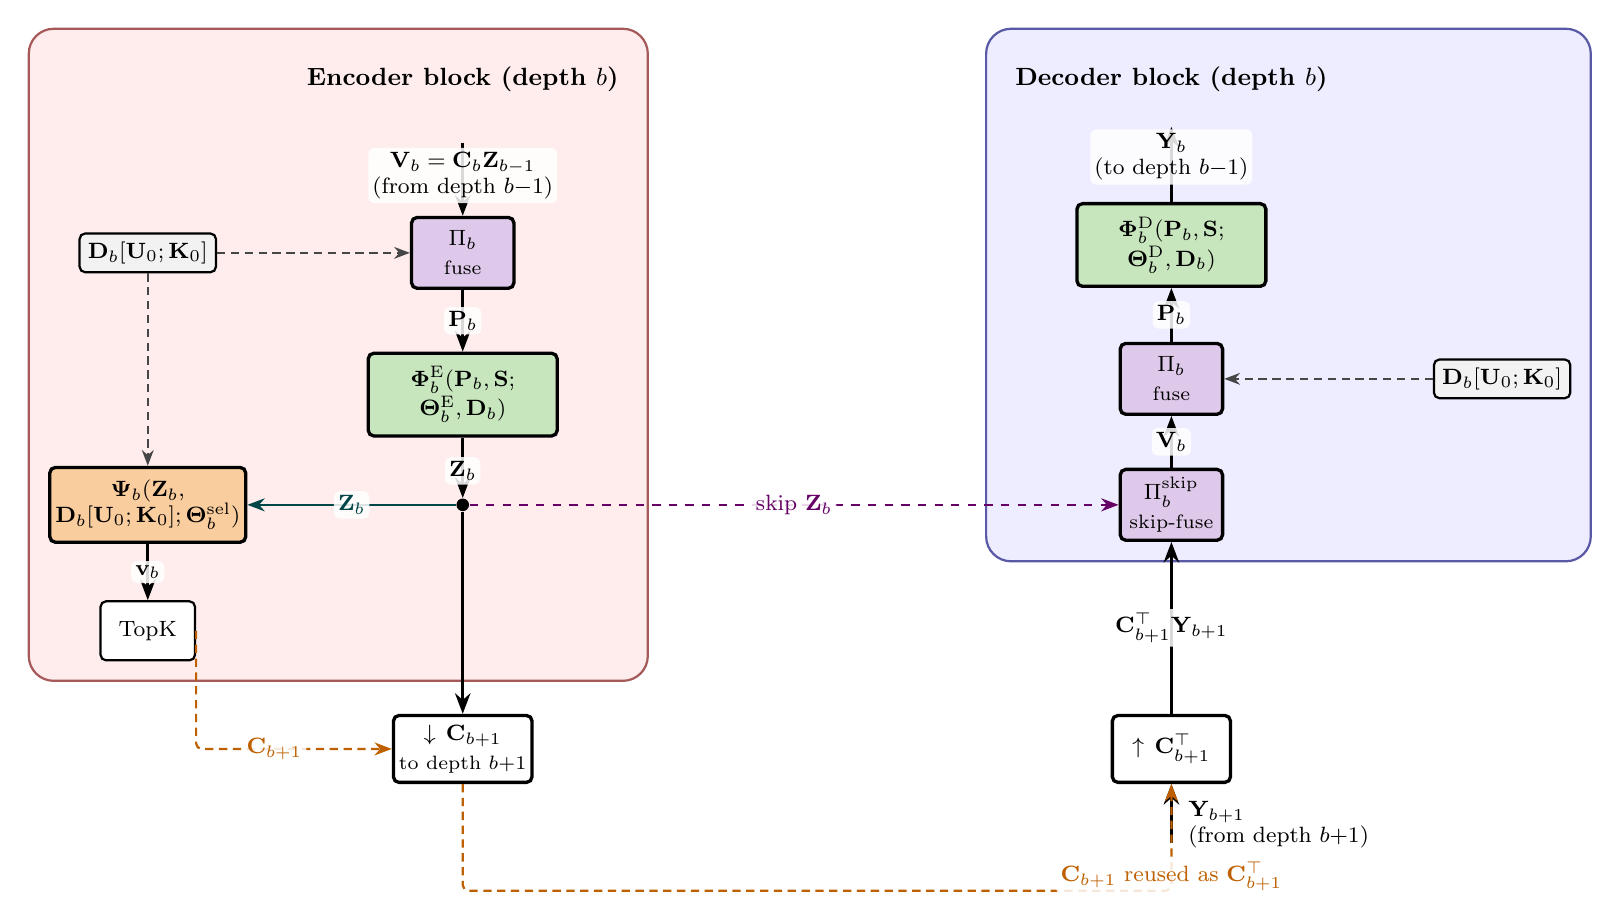
\begin{tikzpicture}[
  >={Stealth[length=2.6mm]},
  rounded corners=2pt,
  proc/.style    = {draw, very thick, rounded corners=2pt, align=center,
                    minimum width=2.4cm, minimum height=1.05cm, inner sep=2pt,
                    font=\footnotesize, fill=gnncol},   % GNN green
  fuseb/.style   = {draw, very thick, rounded corners=2pt, align=center,
                    minimum width=1.3cm, minimum height=0.9cm, inner sep=2pt,
                    font=\footnotesize, fill=projcol},  % projection amber
  encbg/.style   = {rounded corners=9pt, fill=red!7,  draw=red!30!gray, thick,
                    inner sep=7pt},
  decbg/.style   = {rounded corners=9pt, fill=blue!7, draw=blue!30!gray, thick,
                    inner sep=7pt},
  selb/.style    = {draw, very thick, rounded corners=2pt, align=center,
                    minimum width=2.4cm, minimum height=0.95cm, inner sep=2pt,
                    font=\footnotesize, fill=selcol},
  sampb/.style   = {draw, very thick, rounded corners=2pt, align=center,
                    minimum width=1.5cm, minimum height=0.85cm, inner sep=2pt,
                    font=\footnotesize, fill=white},
  condb/.style   = {draw, thick, rounded corners=2pt, align=center,
                    inner sep=3pt, font=\footnotesize, fill=black!5},
  topkb/.style   = {draw, thick, rounded corners=2pt, align=center,
                    minimum width=1.2cm, minimum height=0.75cm, inner sep=2pt,
                    font=\footnotesize, fill=white},
  splitdot/.style= {circle, fill=black, inner sep=0pt, minimum size=1.6mm},
  sig/.style     = {-{Stealth[length=2.6mm]}, very thick},
  feat/.style    = {-{Stealth[length=2.2mm]}, thick, teal!55!black},
  ctrl/.style    = {-{Stealth[length=2.2mm]}, thick, densely dashed, orange!75!black},
  skip/.style    = {-{Stealth[length=2.2mm]}, thick, dashed, violet!80!black},
  condarr/.style = {-{Stealth[length=2.0mm]}, thick, gray!55!black, densely dashed},
  elbl/.style    = {font=\footnotesize, inner sep=1.5pt, fill=white,
                    fill opacity=0.85, text opacity=1},
  hd/.style      = {font=\small\bfseries},
]

% ---------- ENCODER block (depth b) : flows top -> down ----------
\node[fuseb] (Epi)   at (0,6.8) {$\Piblk{b}$\\[1pt]{\scriptsize fuse}};
\node[proc]  (Egnn)  at (0,5.0) {$\PhiEnc{b}(\bbP_b,\bbS;$\\$\thetaenc_b,\bbD_b)$};
\node[splitdot](Esp) at (0,3.6) {};
\node[sampb] (Edown) at (0,0.5) {$\downarrow\,\bbC_{b+1}$\\[1pt]{\scriptsize to depth $b{+}1$}};  % OUTSIDE panel
\node[condb] (Econd) at (-4.0,6.8) {$\bbD_b\UK$};
\node[selb]  (Epsi)  at (-4.0,3.6) {$\Psisel{b}(\bbZ_b,$\\$\bbD_b\UK;\thetasel_{b})$};
\node[topkb] (Etopk) at (-4.0,2.0) {$\mathrm{TopK}$};

\draw[sig]  (0,8.2) -- (Epi.north)
            node[elbl,pos=0.45,align=center]{$\bbV_b=\bbC_b\bbZ_{b-1}$\\(from depth $b{-}1$)};
\draw[condarr] (Econd.east) -- (Epi.west);
\draw[sig]  (Epi.south)  -- (Egnn.north) node[elbl,pos=0.5]{$\bbP_b$};
\draw[sig]  (Egnn.south) -- (Esp)        node[elbl,pos=0.55]{$\bbZ_b$};
\draw[sig]  (Esp) -- (Edown.north);
\draw[feat] (Esp) -- (Epsi.east)         node[elbl,pos=0.5]{$\bbZ_b$};
\draw[condarr] (Econd.south) -- (Epsi.north);
\draw[sig]  (Epsi.south) -- (Etopk.north) node[elbl,pos=0.5]{$\bbvv_{b}$};
\draw[ctrl] (Etopk.east) |- (Edown.west)  node[elbl,pos=0.7]{$\bbC_{b+1}$};

% ---------- DECODER block (depth b) : flows bottom -> up ----------
\node[sampb] (Dup)   at (9,0.5) {$\uparrow\,\bbC_{b+1}^{\top}$};  % OUTSIDE panel
\node[fuseb] (Dskip) at (9,3.6) {$\Piskip{b}$\\[1pt]{\scriptsize skip-fuse}};
\node[fuseb] (Dpi)   at (9,5.2) {$\Piblk{b}$\\[1pt]{\scriptsize fuse}};
\node[proc]  (Dgnn)  at (9,6.9) {$\PhiDec{b}(\bbP_b,\bbS;$\\$\thetadec_b,\bbD_b)$};
\node[condb] (Dcond) at (13.2,5.2) {$\bbD_b\UK$};

\draw[sig]  (9,-0.7) -- (Dup.south)
            node[elbl,pos=0.32,align=left,anchor=west,xshift=4pt]{$\bbY_{b+1}$\\(from depth $b{+}1$)};
\draw[sig]  (Dup.north)   -- (Dskip.south) node[elbl,pos=0.5]{$\bbC_{b+1}^{\top}\bbY_{b+1}$};
\draw[sig]  (Dskip.north) -- (Dpi.south)   node[elbl,pos=0.5]{$\bbV_b$};
\draw[condarr] (Dcond.west) -- (Dpi.east);
\draw[sig]  (Dpi.north)   -- (Dgnn.south)  node[elbl,pos=0.5]{$\bbP_b$};
\draw[sig]  (Dgnn.north)  -- (9,8.4)
            node[elbl,pos=0.6,align=center]{$\bbY_b$\\(to depth $b{-}1$)};

% ---------- cross-links between the two blocks ----------
% skip Z_b : encoder split -> decoder skip-fusion
\draw[skip] (Esp) -- (Dskip.west) node[elbl,pos=0.5]{skip $\bbZ_b$};
% reuse C_{b+1} : encoder selector -> decoder up-sampling
\draw[ctrl] (Edown.south) -- (0,-1.3) -- (9,-1.3) -- (Dup.south)
            node[elbl,pos=0.32,below]{$\bbC_{b+1}$ reused as $\bbC_{b+1}^{\top}$};

% ---------- headers + caption ----------
\node[hd] (Ehdr) at (0,9.0)  {Encoder block (depth $b$)};
\node[hd] (Dhdr) at (9,9.0)  {Decoder block (depth $b$)};

% ---------- half-panel background tints (light red / light blue) ----------
\begin{scope}[on background layer]
  \node[encbg, fit={(Ehdr)(Econd)(Epi)(Egnn)(Esp)(Epsi)(Etopk)(0,9.4)}] {};
  \node[decbg, fit={(Dhdr)(Dskip)(Dpi)(Dgnn)(Dcond)(9,9.4)}] {};
\end{scope}

\ifshowcaption
\node[font=\small, align=center] at (4.5,-2.3)
  {\textbf{Fig.~2.} Block interface. The fusion layer $\Piblk{b}$ is shared across the
   matched encoder/decoder pair; the selection matrix $\bbC_{b+1}$ produced by
   $\Psisel{b}$ on the encoder side is reused (transposed) by the decoder's
   up-sampling. Global embeddings enter as $\bbD_b\UK$.};
\fi

\end{tikzpicture}

\end{document}
"
% Guarded so a double \input cannot redefine/reset the flag.
\ifdefined\ifshowcaption\else \newif\ifshowcaption \showcaptiontrue \fi
\ifdefined\nocaption\showcaptionfalse\fi

%     \showcaptionfalse            % paper supplies its own \caption{}
%  body:
%     \begin{figure*}[t]\centering
%       \resizebox{\textwidth}{!}{\input{path/to/ugnn_fig1}}
%       \caption{...}\label{fig:ugnn}
%     \end{figure*}
%     \begin{figure*}[t]\centering
%       \resizebox{\textwidth}{!}{% ugnn_fig2.tex -- Fig 2 body (block-interface inset). Drawing only.
% \input AFTER _ugnn_preamble.tex.
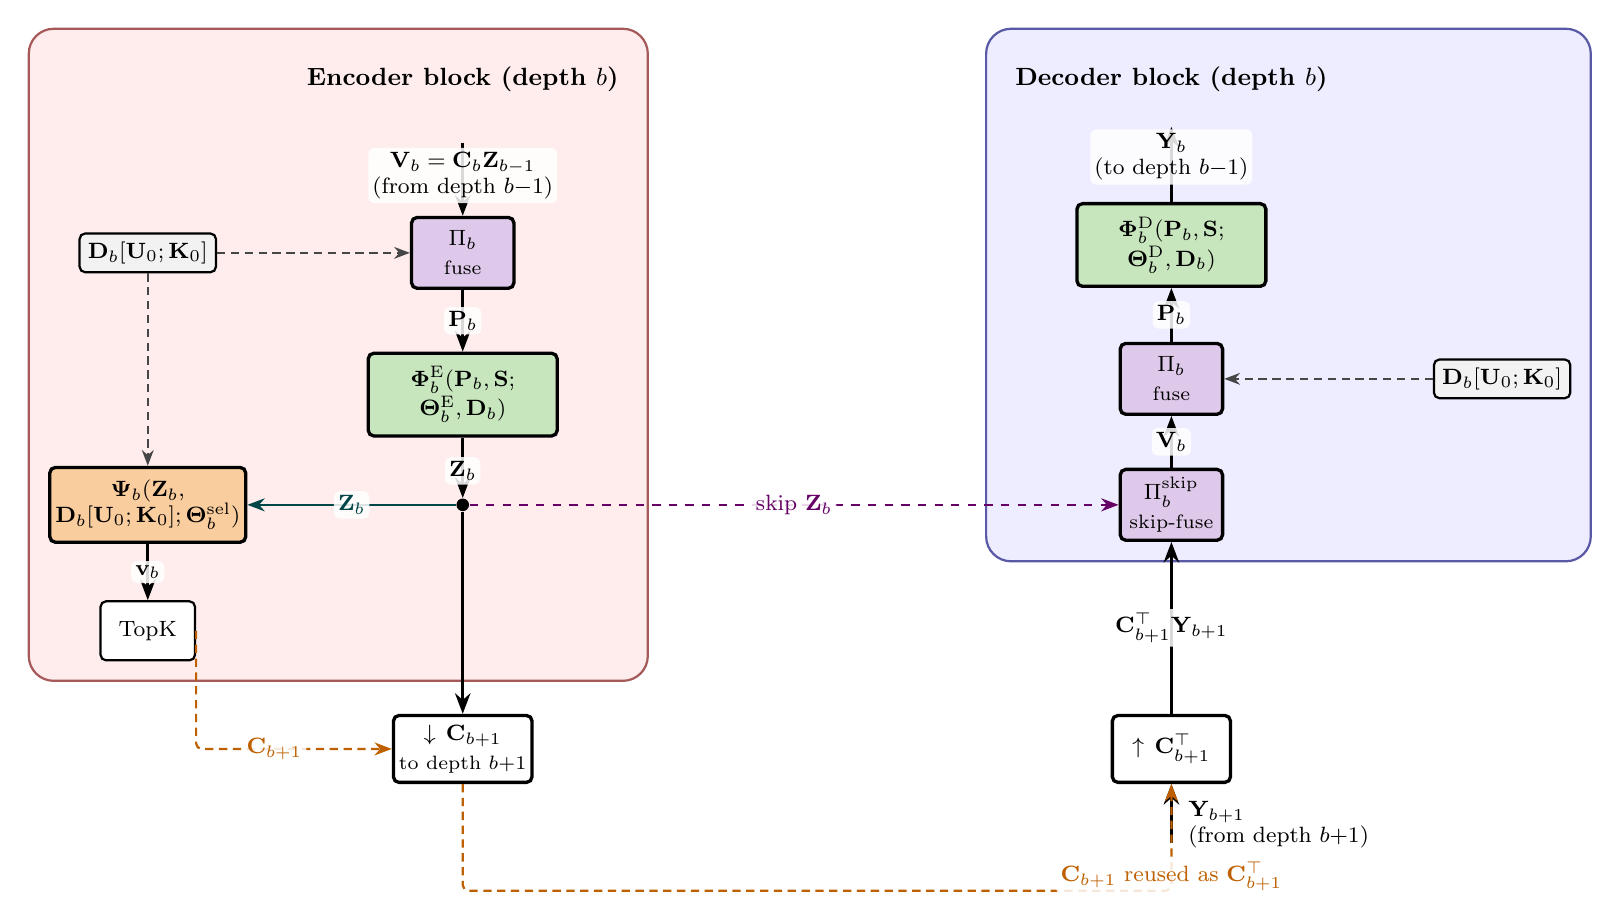
\begin{tikzpicture}[
  >={Stealth[length=2.6mm]},
  rounded corners=2pt,
  proc/.style    = {draw, very thick, rounded corners=2pt, align=center,
                    minimum width=2.4cm, minimum height=1.05cm, inner sep=2pt,
                    font=\footnotesize, fill=gnncol},   % GNN green
  fuseb/.style   = {draw, very thick, rounded corners=2pt, align=center,
                    minimum width=1.3cm, minimum height=0.9cm, inner sep=2pt,
                    font=\footnotesize, fill=projcol},  % projection amber
  encbg/.style   = {rounded corners=9pt, fill=red!7,  draw=red!30!gray, thick,
                    inner sep=7pt},
  decbg/.style   = {rounded corners=9pt, fill=blue!7, draw=blue!30!gray, thick,
                    inner sep=7pt},
  selb/.style    = {draw, very thick, rounded corners=2pt, align=center,
                    minimum width=2.4cm, minimum height=0.95cm, inner sep=2pt,
                    font=\footnotesize, fill=selcol},
  sampb/.style   = {draw, very thick, rounded corners=2pt, align=center,
                    minimum width=1.5cm, minimum height=0.85cm, inner sep=2pt,
                    font=\footnotesize, fill=white},
  condb/.style   = {draw, thick, rounded corners=2pt, align=center,
                    inner sep=3pt, font=\footnotesize, fill=black!5},
  topkb/.style   = {draw, thick, rounded corners=2pt, align=center,
                    minimum width=1.2cm, minimum height=0.75cm, inner sep=2pt,
                    font=\footnotesize, fill=white},
  splitdot/.style= {circle, fill=black, inner sep=0pt, minimum size=1.6mm},
  sig/.style     = {-{Stealth[length=2.6mm]}, very thick},
  feat/.style    = {-{Stealth[length=2.2mm]}, thick, teal!55!black},
  ctrl/.style    = {-{Stealth[length=2.2mm]}, thick, densely dashed, orange!75!black},
  skip/.style    = {-{Stealth[length=2.2mm]}, thick, dashed, violet!80!black},
  condarr/.style = {-{Stealth[length=2.0mm]}, thick, gray!55!black, densely dashed},
  elbl/.style    = {font=\footnotesize, inner sep=1.5pt, fill=white,
                    fill opacity=0.85, text opacity=1},
  hd/.style      = {font=\small\bfseries},
]

% ---------- ENCODER block (depth b) : flows top -> down ----------
\node[fuseb] (Epi)   at (0,6.8) {$\Piblk{b}$\\[1pt]{\scriptsize fuse}};
\node[proc]  (Egnn)  at (0,5.0) {$\PhiEnc{b}(\bbP_b,\bbS;$\\$\thetaenc_b,\bbD_b)$};
\node[splitdot](Esp) at (0,3.6) {};
\node[sampb] (Edown) at (0,0.5) {$\downarrow\,\bbC_{b+1}$\\[1pt]{\scriptsize to depth $b{+}1$}};  % OUTSIDE panel
\node[condb] (Econd) at (-4.0,6.8) {$\bbD_b\UK$};
\node[selb]  (Epsi)  at (-4.0,3.6) {$\Psisel{b}(\bbZ_b,$\\$\bbD_b\UK;\thetasel_{b})$};
\node[topkb] (Etopk) at (-4.0,2.0) {$\mathrm{TopK}$};

\draw[sig]  (0,8.2) -- (Epi.north)
            node[elbl,pos=0.45,align=center]{$\bbV_b=\bbC_b\bbZ_{b-1}$\\(from depth $b{-}1$)};
\draw[condarr] (Econd.east) -- (Epi.west);
\draw[sig]  (Epi.south)  -- (Egnn.north) node[elbl,pos=0.5]{$\bbP_b$};
\draw[sig]  (Egnn.south) -- (Esp)        node[elbl,pos=0.55]{$\bbZ_b$};
\draw[sig]  (Esp) -- (Edown.north);
\draw[feat] (Esp) -- (Epsi.east)         node[elbl,pos=0.5]{$\bbZ_b$};
\draw[condarr] (Econd.south) -- (Epsi.north);
\draw[sig]  (Epsi.south) -- (Etopk.north) node[elbl,pos=0.5]{$\bbvv_{b}$};
\draw[ctrl] (Etopk.east) |- (Edown.west)  node[elbl,pos=0.7]{$\bbC_{b+1}$};

% ---------- DECODER block (depth b) : flows bottom -> up ----------
\node[sampb] (Dup)   at (9,0.5) {$\uparrow\,\bbC_{b+1}^{\top}$};  % OUTSIDE panel
\node[fuseb] (Dskip) at (9,3.6) {$\Piskip{b}$\\[1pt]{\scriptsize skip-fuse}};
\node[fuseb] (Dpi)   at (9,5.2) {$\Piblk{b}$\\[1pt]{\scriptsize fuse}};
\node[proc]  (Dgnn)  at (9,6.9) {$\PhiDec{b}(\bbP_b,\bbS;$\\$\thetadec_b,\bbD_b)$};
\node[condb] (Dcond) at (13.2,5.2) {$\bbD_b\UK$};

\draw[sig]  (9,-0.7) -- (Dup.south)
            node[elbl,pos=0.32,align=left,anchor=west,xshift=4pt]{$\bbY_{b+1}$\\(from depth $b{+}1$)};
\draw[sig]  (Dup.north)   -- (Dskip.south) node[elbl,pos=0.5]{$\bbC_{b+1}^{\top}\bbY_{b+1}$};
\draw[sig]  (Dskip.north) -- (Dpi.south)   node[elbl,pos=0.5]{$\bbV_b$};
\draw[condarr] (Dcond.west) -- (Dpi.east);
\draw[sig]  (Dpi.north)   -- (Dgnn.south)  node[elbl,pos=0.5]{$\bbP_b$};
\draw[sig]  (Dgnn.north)  -- (9,8.4)
            node[elbl,pos=0.6,align=center]{$\bbY_b$\\(to depth $b{-}1$)};

% ---------- cross-links between the two blocks ----------
% skip Z_b : encoder split -> decoder skip-fusion
\draw[skip] (Esp) -- (Dskip.west) node[elbl,pos=0.5]{skip $\bbZ_b$};
% reuse C_{b+1} : encoder selector -> decoder up-sampling
\draw[ctrl] (Edown.south) -- (0,-1.3) -- (9,-1.3) -- (Dup.south)
            node[elbl,pos=0.32,below]{$\bbC_{b+1}$ reused as $\bbC_{b+1}^{\top}$};

% ---------- headers + caption ----------
\node[hd] (Ehdr) at (0,9.0)  {Encoder block (depth $b$)};
\node[hd] (Dhdr) at (9,9.0)  {Decoder block (depth $b$)};

% ---------- half-panel background tints (light red / light blue) ----------
\begin{scope}[on background layer]
  \node[encbg, fit={(Ehdr)(Econd)(Epi)(Egnn)(Esp)(Epsi)(Etopk)(0,9.4)}] {};
  \node[decbg, fit={(Dhdr)(Dskip)(Dpi)(Dgnn)(Dcond)(9,9.4)}] {};
\end{scope}

\ifshowcaption
\node[font=\small, align=center] at (4.5,-2.3)
  {\textbf{Fig.~2.} Block interface. The fusion layer $\Piblk{b}$ is shared across the
   matched encoder/decoder pair; the selection matrix $\bbC_{b+1}$ produced by
   $\Psisel{b}$ on the encoder side is reused (transposed) by the decoder's
   up-sampling. Global embeddings enter as $\bbD_b\UK$.};
\fi

\end{tikzpicture}
}
%       \caption{...}\label{fig:ugnn-block}
%     \end{figure*}
%  NB embedded, fonts inherit YOUR paper's class (not extarticle 17pt);
%  \resizebox scales the whole picture, so it stays internally consistent.
% =====================================================================
\usetikzlibrary{arrows.meta, positioning, calc, backgrounds, fit}

% ===== categorical block palette =====================================
%   green  = GNN  (phi^enc / phi^dec / phi^bn)
%   purple = projection layers (Pi_0, Pi^cond, Pi^step, Pi_b, Pi^skip, Pi_out)
%   orange = learned node selector (Psi_b)  -- matches its C_b control edges
%   red / blue are RESERVED for the encoder / decoder panels.
\definecolor{gnncol}{RGB}{200,230,190}
\definecolor{projcol}{RGB}{223,201,234}
\definecolor{selcol}{RGB}{250,205,158}
\definecolor{bandcol}{RGB}{176,130,80}   % depth-band base (warm golden sand; swap freely)

% ===== math glyphs (\providecommand: figure owns them, but a paper that ====
% ===== already defines the symbol keeps its own version, no clash) ========
\providecommand{\bbS}{\mathbf{S}}
\providecommand{\bbC}{\mathbf{C}}
\providecommand{\bbD}{\mathbf{D}}
\providecommand{\bbZ}{\mathbf{Z}}
\providecommand{\bbY}{\mathbf{Y}}
\providecommand{\bbU}{\mathbf{U}}
\providecommand{\bbK}{\mathbf{K}}
\providecommand{\bbP}{\mathbf{P}}
\providecommand{\bbV}{\mathbf{V}}
\providecommand{\bbI}{\mathbf{I}}
\providecommand{\bbvv}{\mathbf{v}}
\providecommand{\bbx}{\mathbf{x}}
\providecommand{\bbu}{\mathbf{u}}
\providecommand{\bbeps}{\boldsymbol{\epsilon}_{\boldsymbol{\theta}}}
\providecommand{\bbepsilon}{\boldsymbol{\epsilon}}      % bare epsilon (subscript supplied at use site)
\providecommand{\bbtheta}{\boldsymbol{\theta}}
\providecommand{\bbxi}{\boldsymbol{\xi}}                % compact conditioning placeholder (S,u,...)
\providecommand{\alphacumprod}{\bar{\alpha}}            % cumulative-product noise schedule constant
\providecommand{\UK}{[\bbU_0;\bbK_0]}
% GNN operators (single symbol phi, role superscript)
\providecommand{\PhiEnc}[1]{\boldsymbol{\Phi}^{\mathrm{E}}_{#1}}
\providecommand{\PhiDec}[1]{\boldsymbol{\Phi}^{\mathrm{D}}_{#1}}
\providecommand{\PhiBn}{\boldsymbol{\Phi}^{\mathrm{B}}}
% projection / embedding family
\providecommand{\Piin}{\Pi_{0}}
\providecommand{\Picond}{\Pi^{\mathrm{cond}}_{0}}
\providecommand{\Pistep}{\Pi^{\mathrm{step}}_{0}}
\providecommand{\Piblk}[1]{\Pi_{#1}}
\providecommand{\Piskip}[1]{\Pi^{\mathrm{skip}}_{#1}}
\providecommand{\Piout}{\Pi_{\mathrm{out}}}
% scoring head
\providecommand{\Psisel}[1]{\boldsymbol{\Psi}_{#1}}
% learnable parameters
\providecommand{\thetaenc}{\boldsymbol{\Theta}^{\mathrm{E}}}
\providecommand{\thetadec}{\boldsymbol{\Theta}^{\mathrm{D}}}
\providecommand{\thetasel}{\boldsymbol{\Theta}^{\mathrm{sel}}}

% ===== caption toggle (build option) =================================
% Captions ON by default.  Turn OFF either way:
%   * after this \input:  \showcaptionfalse        (e.g. when embedding in a paper)
%   * on the command line: pdflatex "\def\nocaption{}% =====================================================================
%  U-GNN denoiser architecture  (reference: oarfish-9)  --  STANDALONE WRAPPER
%
%  This file is now a THIN WRAPPER, used only for local 2-page preview.
%  The actual drawing code lives in three sibling files:
%      _ugnn_preamble.tex  -- shared colours, glyph macros, caption toggle
%      ugnn_fig1.tex       -- Fig 1 (high-level encoder-decoder U)
%      ugnn_fig2.tex       -- Fig 2 (block-interface inset)
%  To EMBED the figures in a paper, \input the preamble + each body file
%  directly into your main.tex (see the header of _ugnn_preamble.tex for the
%  exact snippet); do NOT \input this wrapper.
%
%  Notation (single GNN symbol phi; conditioning fused by Pi_b before phi):
%    encoder    Z_b   = Phi^E_b ( P_b , S ; Theta^enc_b , D_b )
%    decoder    Y_b   = Phi^D_b ( P_b , S ; Theta^dec_b , D_b )
%    bottleneck Y_{B+1}= Phi^B  ( C_{B+1} Z_B , S ; Theta^bn , D_{B+1} )
%    block fuse P_b   = Pi_b ( V_b , D_b [U_0;K_0] )
%    selection (depth-b selector)  v_b = Psi_b ( Z_b , D_b[U_0;K_0] ) ; C_{b+1} = TopK(v_b)
%
%  Compile (with captions):  pdflatex ugnn_architecture_full.tex
%  Compile (no captions):    pdflatex "\def\nocaption{}% =====================================================================
%  U-GNN denoiser architecture  (reference: oarfish-9)  --  STANDALONE WRAPPER
%
%  This file is now a THIN WRAPPER, used only for local 2-page preview.
%  The actual drawing code lives in three sibling files:
%      _ugnn_preamble.tex  -- shared colours, glyph macros, caption toggle
%      ugnn_fig1.tex       -- Fig 1 (high-level encoder-decoder U)
%      ugnn_fig2.tex       -- Fig 2 (block-interface inset)
%  To EMBED the figures in a paper, \input the preamble + each body file
%  directly into your main.tex (see the header of _ugnn_preamble.tex for the
%  exact snippet); do NOT \input this wrapper.
%
%  Notation (single GNN symbol phi; conditioning fused by Pi_b before phi):
%    encoder    Z_b   = Phi^E_b ( P_b , S ; Theta^enc_b , D_b )
%    decoder    Y_b   = Phi^D_b ( P_b , S ; Theta^dec_b , D_b )
%    bottleneck Y_{B+1}= Phi^B  ( C_{B+1} Z_B , S ; Theta^bn , D_{B+1} )
%    block fuse P_b   = Pi_b ( V_b , D_b [U_0;K_0] )
%    selection (depth-b selector)  v_b = Psi_b ( Z_b , D_b[U_0;K_0] ) ; C_{b+1} = TopK(v_b)
%
%  Compile (with captions):  pdflatex ugnn_architecture_full.tex
%  Compile (no captions):    pdflatex "\def\nocaption{}% =====================================================================
%  U-GNN denoiser architecture  (reference: oarfish-9)  --  STANDALONE WRAPPER
%
%  This file is now a THIN WRAPPER, used only for local 2-page preview.
%  The actual drawing code lives in three sibling files:
%      _ugnn_preamble.tex  -- shared colours, glyph macros, caption toggle
%      ugnn_fig1.tex       -- Fig 1 (high-level encoder-decoder U)
%      ugnn_fig2.tex       -- Fig 2 (block-interface inset)
%  To EMBED the figures in a paper, \input the preamble + each body file
%  directly into your main.tex (see the header of _ugnn_preamble.tex for the
%  exact snippet); do NOT \input this wrapper.
%
%  Notation (single GNN symbol phi; conditioning fused by Pi_b before phi):
%    encoder    Z_b   = Phi^E_b ( P_b , S ; Theta^enc_b , D_b )
%    decoder    Y_b   = Phi^D_b ( P_b , S ; Theta^dec_b , D_b )
%    bottleneck Y_{B+1}= Phi^B  ( C_{B+1} Z_B , S ; Theta^bn , D_{B+1} )
%    block fuse P_b   = Pi_b ( V_b , D_b [U_0;K_0] )
%    selection (depth-b selector)  v_b = Psi_b ( Z_b , D_b[U_0;K_0] ) ; C_{b+1} = TopK(v_b)
%
%  Compile (with captions):  pdflatex ugnn_architecture_full.tex
%  Compile (no captions):    pdflatex "\def\nocaption{}\input{ugnn_architecture_full}"
% =====================================================================
\documentclass[tikz,border=12pt,class=extarticle,17pt]{standalone}   % extarticle 17pt base: bigger global fonts
\usepackage{amsmath}
\input{_ugnn_preamble}

\begin{document}
\input{ugnn_fig1}
\newpage
\input{ugnn_fig2}
\end{document}
"
% =====================================================================
\documentclass[tikz,border=12pt,class=extarticle,17pt]{standalone}   % extarticle 17pt base: bigger global fonts
\usepackage{amsmath}
% =====================================================================
%  _ugnn_preamble.tex  --  SHARED preamble fragment for the U-GNN figures
%  (reference: oarfish-9)
%
%  \input this ONCE, in the PREAMBLE, from EITHER:
%    * the standalone wrapper  ugnn_architecture_full.tex  (local 2-page preview), OR
%    * your paper's main.tex   (to embed ugnn_fig1.tex / ugnn_fig2.tex).
%
%  Provides: TikZ libraries, the categorical colour palette, every math glyph
%  macro (\bb*, \Phi*, \Pi*, \Psi*, \theta*), and the caption toggle.  The glyph
%  macros use \providecommand, so if your paper ALREADY defines e.g. \bbS, your
%  definition wins and nothing clashes.
%
%  REQUIRES tikz + amsmath already loaded (tikz pulls in xcolor for \definecolor).
%
%  ---- paper-side usage -------------------------------------------------
%  preamble:
%     \usepackage{tikz}\usepackage{amsmath}\usepackage{graphicx}
%     \input{path/to/_ugnn_preamble}
%     \showcaptionfalse            % paper supplies its own \caption{}
%  body:
%     \begin{figure*}[t]\centering
%       \resizebox{\textwidth}{!}{\input{path/to/ugnn_fig1}}
%       \caption{...}\label{fig:ugnn}
%     \end{figure*}
%     \begin{figure*}[t]\centering
%       \resizebox{\textwidth}{!}{\input{path/to/ugnn_fig2}}
%       \caption{...}\label{fig:ugnn-block}
%     \end{figure*}
%  NB embedded, fonts inherit YOUR paper's class (not extarticle 17pt);
%  \resizebox scales the whole picture, so it stays internally consistent.
% =====================================================================
\usetikzlibrary{arrows.meta, positioning, calc, backgrounds, fit}

% ===== categorical block palette =====================================
%   green  = GNN  (phi^enc / phi^dec / phi^bn)
%   purple = projection layers (Pi_0, Pi^cond, Pi^step, Pi_b, Pi^skip, Pi_out)
%   orange = learned node selector (Psi_b)  -- matches its C_b control edges
%   red / blue are RESERVED for the encoder / decoder panels.
\definecolor{gnncol}{RGB}{200,230,190}
\definecolor{projcol}{RGB}{223,201,234}
\definecolor{selcol}{RGB}{250,205,158}
\definecolor{bandcol}{RGB}{176,130,80}   % depth-band base (warm golden sand; swap freely)

% ===== math glyphs (\providecommand: figure owns them, but a paper that ====
% ===== already defines the symbol keeps its own version, no clash) ========
\providecommand{\bbS}{\mathbf{S}}
\providecommand{\bbC}{\mathbf{C}}
\providecommand{\bbD}{\mathbf{D}}
\providecommand{\bbZ}{\mathbf{Z}}
\providecommand{\bbY}{\mathbf{Y}}
\providecommand{\bbU}{\mathbf{U}}
\providecommand{\bbK}{\mathbf{K}}
\providecommand{\bbP}{\mathbf{P}}
\providecommand{\bbV}{\mathbf{V}}
\providecommand{\bbI}{\mathbf{I}}
\providecommand{\bbvv}{\mathbf{v}}
\providecommand{\bbx}{\mathbf{x}}
\providecommand{\bbu}{\mathbf{u}}
\providecommand{\bbeps}{\boldsymbol{\epsilon}_{\boldsymbol{\theta}}}
\providecommand{\bbepsilon}{\boldsymbol{\epsilon}}      % bare epsilon (subscript supplied at use site)
\providecommand{\bbtheta}{\boldsymbol{\theta}}
\providecommand{\bbxi}{\boldsymbol{\xi}}                % compact conditioning placeholder (S,u,...)
\providecommand{\alphacumprod}{\bar{\alpha}}            % cumulative-product noise schedule constant
\providecommand{\UK}{[\bbU_0;\bbK_0]}
% GNN operators (single symbol phi, role superscript)
\providecommand{\PhiEnc}[1]{\boldsymbol{\Phi}^{\mathrm{E}}_{#1}}
\providecommand{\PhiDec}[1]{\boldsymbol{\Phi}^{\mathrm{D}}_{#1}}
\providecommand{\PhiBn}{\boldsymbol{\Phi}^{\mathrm{B}}}
% projection / embedding family
\providecommand{\Piin}{\Pi_{0}}
\providecommand{\Picond}{\Pi^{\mathrm{cond}}_{0}}
\providecommand{\Pistep}{\Pi^{\mathrm{step}}_{0}}
\providecommand{\Piblk}[1]{\Pi_{#1}}
\providecommand{\Piskip}[1]{\Pi^{\mathrm{skip}}_{#1}}
\providecommand{\Piout}{\Pi_{\mathrm{out}}}
% scoring head
\providecommand{\Psisel}[1]{\boldsymbol{\Psi}_{#1}}
% learnable parameters
\providecommand{\thetaenc}{\boldsymbol{\Theta}^{\mathrm{E}}}
\providecommand{\thetadec}{\boldsymbol{\Theta}^{\mathrm{D}}}
\providecommand{\thetasel}{\boldsymbol{\Theta}^{\mathrm{sel}}}

% ===== caption toggle (build option) =================================
% Captions ON by default.  Turn OFF either way:
%   * after this \input:  \showcaptionfalse        (e.g. when embedding in a paper)
%   * on the command line: pdflatex "\def\nocaption{}\input{ugnn_architecture_full}"
% Guarded so a double \input cannot redefine/reset the flag.
\ifdefined\ifshowcaption\else \newif\ifshowcaption \showcaptiontrue \fi
\ifdefined\nocaption\showcaptionfalse\fi


\begin{document}
\input{ugnn_fig1}
\newpage
% ugnn_fig2.tex -- Fig 2 body (block-interface inset). Drawing only.
% \input AFTER _ugnn_preamble.tex.
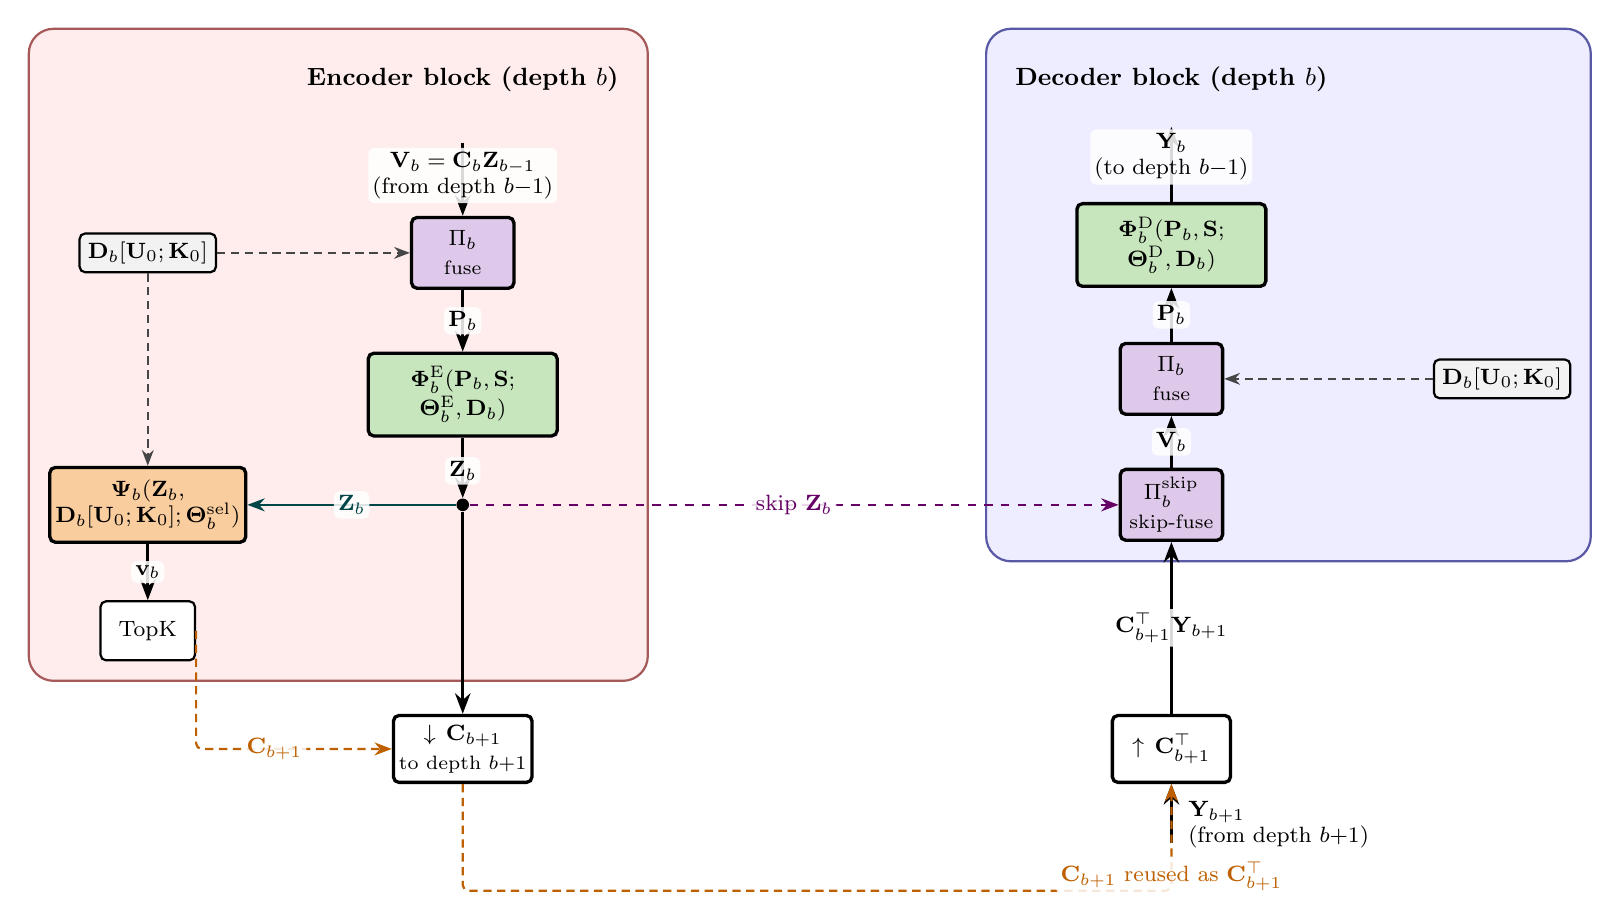
\begin{tikzpicture}[
  >={Stealth[length=2.6mm]},
  rounded corners=2pt,
  proc/.style    = {draw, very thick, rounded corners=2pt, align=center,
                    minimum width=2.4cm, minimum height=1.05cm, inner sep=2pt,
                    font=\footnotesize, fill=gnncol},   % GNN green
  fuseb/.style   = {draw, very thick, rounded corners=2pt, align=center,
                    minimum width=1.3cm, minimum height=0.9cm, inner sep=2pt,
                    font=\footnotesize, fill=projcol},  % projection amber
  encbg/.style   = {rounded corners=9pt, fill=red!7,  draw=red!30!gray, thick,
                    inner sep=7pt},
  decbg/.style   = {rounded corners=9pt, fill=blue!7, draw=blue!30!gray, thick,
                    inner sep=7pt},
  selb/.style    = {draw, very thick, rounded corners=2pt, align=center,
                    minimum width=2.4cm, minimum height=0.95cm, inner sep=2pt,
                    font=\footnotesize, fill=selcol},
  sampb/.style   = {draw, very thick, rounded corners=2pt, align=center,
                    minimum width=1.5cm, minimum height=0.85cm, inner sep=2pt,
                    font=\footnotesize, fill=white},
  condb/.style   = {draw, thick, rounded corners=2pt, align=center,
                    inner sep=3pt, font=\footnotesize, fill=black!5},
  topkb/.style   = {draw, thick, rounded corners=2pt, align=center,
                    minimum width=1.2cm, minimum height=0.75cm, inner sep=2pt,
                    font=\footnotesize, fill=white},
  splitdot/.style= {circle, fill=black, inner sep=0pt, minimum size=1.6mm},
  sig/.style     = {-{Stealth[length=2.6mm]}, very thick},
  feat/.style    = {-{Stealth[length=2.2mm]}, thick, teal!55!black},
  ctrl/.style    = {-{Stealth[length=2.2mm]}, thick, densely dashed, orange!75!black},
  skip/.style    = {-{Stealth[length=2.2mm]}, thick, dashed, violet!80!black},
  condarr/.style = {-{Stealth[length=2.0mm]}, thick, gray!55!black, densely dashed},
  elbl/.style    = {font=\footnotesize, inner sep=1.5pt, fill=white,
                    fill opacity=0.85, text opacity=1},
  hd/.style      = {font=\small\bfseries},
]

% ---------- ENCODER block (depth b) : flows top -> down ----------
\node[fuseb] (Epi)   at (0,6.8) {$\Piblk{b}$\\[1pt]{\scriptsize fuse}};
\node[proc]  (Egnn)  at (0,5.0) {$\PhiEnc{b}(\bbP_b,\bbS;$\\$\thetaenc_b,\bbD_b)$};
\node[splitdot](Esp) at (0,3.6) {};
\node[sampb] (Edown) at (0,0.5) {$\downarrow\,\bbC_{b+1}$\\[1pt]{\scriptsize to depth $b{+}1$}};  % OUTSIDE panel
\node[condb] (Econd) at (-4.0,6.8) {$\bbD_b\UK$};
\node[selb]  (Epsi)  at (-4.0,3.6) {$\Psisel{b}(\bbZ_b,$\\$\bbD_b\UK;\thetasel_{b})$};
\node[topkb] (Etopk) at (-4.0,2.0) {$\mathrm{TopK}$};

\draw[sig]  (0,8.2) -- (Epi.north)
            node[elbl,pos=0.45,align=center]{$\bbV_b=\bbC_b\bbZ_{b-1}$\\(from depth $b{-}1$)};
\draw[condarr] (Econd.east) -- (Epi.west);
\draw[sig]  (Epi.south)  -- (Egnn.north) node[elbl,pos=0.5]{$\bbP_b$};
\draw[sig]  (Egnn.south) -- (Esp)        node[elbl,pos=0.55]{$\bbZ_b$};
\draw[sig]  (Esp) -- (Edown.north);
\draw[feat] (Esp) -- (Epsi.east)         node[elbl,pos=0.5]{$\bbZ_b$};
\draw[condarr] (Econd.south) -- (Epsi.north);
\draw[sig]  (Epsi.south) -- (Etopk.north) node[elbl,pos=0.5]{$\bbvv_{b}$};
\draw[ctrl] (Etopk.east) |- (Edown.west)  node[elbl,pos=0.7]{$\bbC_{b+1}$};

% ---------- DECODER block (depth b) : flows bottom -> up ----------
\node[sampb] (Dup)   at (9,0.5) {$\uparrow\,\bbC_{b+1}^{\top}$};  % OUTSIDE panel
\node[fuseb] (Dskip) at (9,3.6) {$\Piskip{b}$\\[1pt]{\scriptsize skip-fuse}};
\node[fuseb] (Dpi)   at (9,5.2) {$\Piblk{b}$\\[1pt]{\scriptsize fuse}};
\node[proc]  (Dgnn)  at (9,6.9) {$\PhiDec{b}(\bbP_b,\bbS;$\\$\thetadec_b,\bbD_b)$};
\node[condb] (Dcond) at (13.2,5.2) {$\bbD_b\UK$};

\draw[sig]  (9,-0.7) -- (Dup.south)
            node[elbl,pos=0.32,align=left,anchor=west,xshift=4pt]{$\bbY_{b+1}$\\(from depth $b{+}1$)};
\draw[sig]  (Dup.north)   -- (Dskip.south) node[elbl,pos=0.5]{$\bbC_{b+1}^{\top}\bbY_{b+1}$};
\draw[sig]  (Dskip.north) -- (Dpi.south)   node[elbl,pos=0.5]{$\bbV_b$};
\draw[condarr] (Dcond.west) -- (Dpi.east);
\draw[sig]  (Dpi.north)   -- (Dgnn.south)  node[elbl,pos=0.5]{$\bbP_b$};
\draw[sig]  (Dgnn.north)  -- (9,8.4)
            node[elbl,pos=0.6,align=center]{$\bbY_b$\\(to depth $b{-}1$)};

% ---------- cross-links between the two blocks ----------
% skip Z_b : encoder split -> decoder skip-fusion
\draw[skip] (Esp) -- (Dskip.west) node[elbl,pos=0.5]{skip $\bbZ_b$};
% reuse C_{b+1} : encoder selector -> decoder up-sampling
\draw[ctrl] (Edown.south) -- (0,-1.3) -- (9,-1.3) -- (Dup.south)
            node[elbl,pos=0.32,below]{$\bbC_{b+1}$ reused as $\bbC_{b+1}^{\top}$};

% ---------- headers + caption ----------
\node[hd] (Ehdr) at (0,9.0)  {Encoder block (depth $b$)};
\node[hd] (Dhdr) at (9,9.0)  {Decoder block (depth $b$)};

% ---------- half-panel background tints (light red / light blue) ----------
\begin{scope}[on background layer]
  \node[encbg, fit={(Ehdr)(Econd)(Epi)(Egnn)(Esp)(Epsi)(Etopk)(0,9.4)}] {};
  \node[decbg, fit={(Dhdr)(Dskip)(Dpi)(Dgnn)(Dcond)(9,9.4)}] {};
\end{scope}

\ifshowcaption
\node[font=\small, align=center] at (4.5,-2.3)
  {\textbf{Fig.~2.} Block interface. The fusion layer $\Piblk{b}$ is shared across the
   matched encoder/decoder pair; the selection matrix $\bbC_{b+1}$ produced by
   $\Psisel{b}$ on the encoder side is reused (transposed) by the decoder's
   up-sampling. Global embeddings enter as $\bbD_b\UK$.};
\fi

\end{tikzpicture}

\end{document}
"
% =====================================================================
\documentclass[tikz,border=12pt,class=extarticle,17pt]{standalone}   % extarticle 17pt base: bigger global fonts
\usepackage{amsmath}
% =====================================================================
%  _ugnn_preamble.tex  --  SHARED preamble fragment for the U-GNN figures
%  (reference: oarfish-9)
%
%  \input this ONCE, in the PREAMBLE, from EITHER:
%    * the standalone wrapper  ugnn_architecture_full.tex  (local 2-page preview), OR
%    * your paper's main.tex   (to embed ugnn_fig1.tex / ugnn_fig2.tex).
%
%  Provides: TikZ libraries, the categorical colour palette, every math glyph
%  macro (\bb*, \Phi*, \Pi*, \Psi*, \theta*), and the caption toggle.  The glyph
%  macros use \providecommand, so if your paper ALREADY defines e.g. \bbS, your
%  definition wins and nothing clashes.
%
%  REQUIRES tikz + amsmath already loaded (tikz pulls in xcolor for \definecolor).
%
%  ---- paper-side usage -------------------------------------------------
%  preamble:
%     \usepackage{tikz}\usepackage{amsmath}\usepackage{graphicx}
%     % =====================================================================
%  _ugnn_preamble.tex  --  SHARED preamble fragment for the U-GNN figures
%  (reference: oarfish-9)
%
%  \input this ONCE, in the PREAMBLE, from EITHER:
%    * the standalone wrapper  ugnn_architecture_full.tex  (local 2-page preview), OR
%    * your paper's main.tex   (to embed ugnn_fig1.tex / ugnn_fig2.tex).
%
%  Provides: TikZ libraries, the categorical colour palette, every math glyph
%  macro (\bb*, \Phi*, \Pi*, \Psi*, \theta*), and the caption toggle.  The glyph
%  macros use \providecommand, so if your paper ALREADY defines e.g. \bbS, your
%  definition wins and nothing clashes.
%
%  REQUIRES tikz + amsmath already loaded (tikz pulls in xcolor for \definecolor).
%
%  ---- paper-side usage -------------------------------------------------
%  preamble:
%     \usepackage{tikz}\usepackage{amsmath}\usepackage{graphicx}
%     \input{path/to/_ugnn_preamble}
%     \showcaptionfalse            % paper supplies its own \caption{}
%  body:
%     \begin{figure*}[t]\centering
%       \resizebox{\textwidth}{!}{\input{path/to/ugnn_fig1}}
%       \caption{...}\label{fig:ugnn}
%     \end{figure*}
%     \begin{figure*}[t]\centering
%       \resizebox{\textwidth}{!}{\input{path/to/ugnn_fig2}}
%       \caption{...}\label{fig:ugnn-block}
%     \end{figure*}
%  NB embedded, fonts inherit YOUR paper's class (not extarticle 17pt);
%  \resizebox scales the whole picture, so it stays internally consistent.
% =====================================================================
\usetikzlibrary{arrows.meta, positioning, calc, backgrounds, fit}

% ===== categorical block palette =====================================
%   green  = GNN  (phi^enc / phi^dec / phi^bn)
%   purple = projection layers (Pi_0, Pi^cond, Pi^step, Pi_b, Pi^skip, Pi_out)
%   orange = learned node selector (Psi_b)  -- matches its C_b control edges
%   red / blue are RESERVED for the encoder / decoder panels.
\definecolor{gnncol}{RGB}{200,230,190}
\definecolor{projcol}{RGB}{223,201,234}
\definecolor{selcol}{RGB}{250,205,158}
\definecolor{bandcol}{RGB}{176,130,80}   % depth-band base (warm golden sand; swap freely)

% ===== math glyphs (\providecommand: figure owns them, but a paper that ====
% ===== already defines the symbol keeps its own version, no clash) ========
\providecommand{\bbS}{\mathbf{S}}
\providecommand{\bbC}{\mathbf{C}}
\providecommand{\bbD}{\mathbf{D}}
\providecommand{\bbZ}{\mathbf{Z}}
\providecommand{\bbY}{\mathbf{Y}}
\providecommand{\bbU}{\mathbf{U}}
\providecommand{\bbK}{\mathbf{K}}
\providecommand{\bbP}{\mathbf{P}}
\providecommand{\bbV}{\mathbf{V}}
\providecommand{\bbI}{\mathbf{I}}
\providecommand{\bbvv}{\mathbf{v}}
\providecommand{\bbx}{\mathbf{x}}
\providecommand{\bbu}{\mathbf{u}}
\providecommand{\bbeps}{\boldsymbol{\epsilon}_{\boldsymbol{\theta}}}
\providecommand{\bbepsilon}{\boldsymbol{\epsilon}}      % bare epsilon (subscript supplied at use site)
\providecommand{\bbtheta}{\boldsymbol{\theta}}
\providecommand{\bbxi}{\boldsymbol{\xi}}                % compact conditioning placeholder (S,u,...)
\providecommand{\alphacumprod}{\bar{\alpha}}            % cumulative-product noise schedule constant
\providecommand{\UK}{[\bbU_0;\bbK_0]}
% GNN operators (single symbol phi, role superscript)
\providecommand{\PhiEnc}[1]{\boldsymbol{\Phi}^{\mathrm{E}}_{#1}}
\providecommand{\PhiDec}[1]{\boldsymbol{\Phi}^{\mathrm{D}}_{#1}}
\providecommand{\PhiBn}{\boldsymbol{\Phi}^{\mathrm{B}}}
% projection / embedding family
\providecommand{\Piin}{\Pi_{0}}
\providecommand{\Picond}{\Pi^{\mathrm{cond}}_{0}}
\providecommand{\Pistep}{\Pi^{\mathrm{step}}_{0}}
\providecommand{\Piblk}[1]{\Pi_{#1}}
\providecommand{\Piskip}[1]{\Pi^{\mathrm{skip}}_{#1}}
\providecommand{\Piout}{\Pi_{\mathrm{out}}}
% scoring head
\providecommand{\Psisel}[1]{\boldsymbol{\Psi}_{#1}}
% learnable parameters
\providecommand{\thetaenc}{\boldsymbol{\Theta}^{\mathrm{E}}}
\providecommand{\thetadec}{\boldsymbol{\Theta}^{\mathrm{D}}}
\providecommand{\thetasel}{\boldsymbol{\Theta}^{\mathrm{sel}}}

% ===== caption toggle (build option) =================================
% Captions ON by default.  Turn OFF either way:
%   * after this \input:  \showcaptionfalse        (e.g. when embedding in a paper)
%   * on the command line: pdflatex "\def\nocaption{}\input{ugnn_architecture_full}"
% Guarded so a double \input cannot redefine/reset the flag.
\ifdefined\ifshowcaption\else \newif\ifshowcaption \showcaptiontrue \fi
\ifdefined\nocaption\showcaptionfalse\fi

%     \showcaptionfalse            % paper supplies its own \caption{}
%  body:
%     \begin{figure*}[t]\centering
%       \resizebox{\textwidth}{!}{\input{path/to/ugnn_fig1}}
%       \caption{...}\label{fig:ugnn}
%     \end{figure*}
%     \begin{figure*}[t]\centering
%       \resizebox{\textwidth}{!}{% ugnn_fig2.tex -- Fig 2 body (block-interface inset). Drawing only.
% \input AFTER _ugnn_preamble.tex.
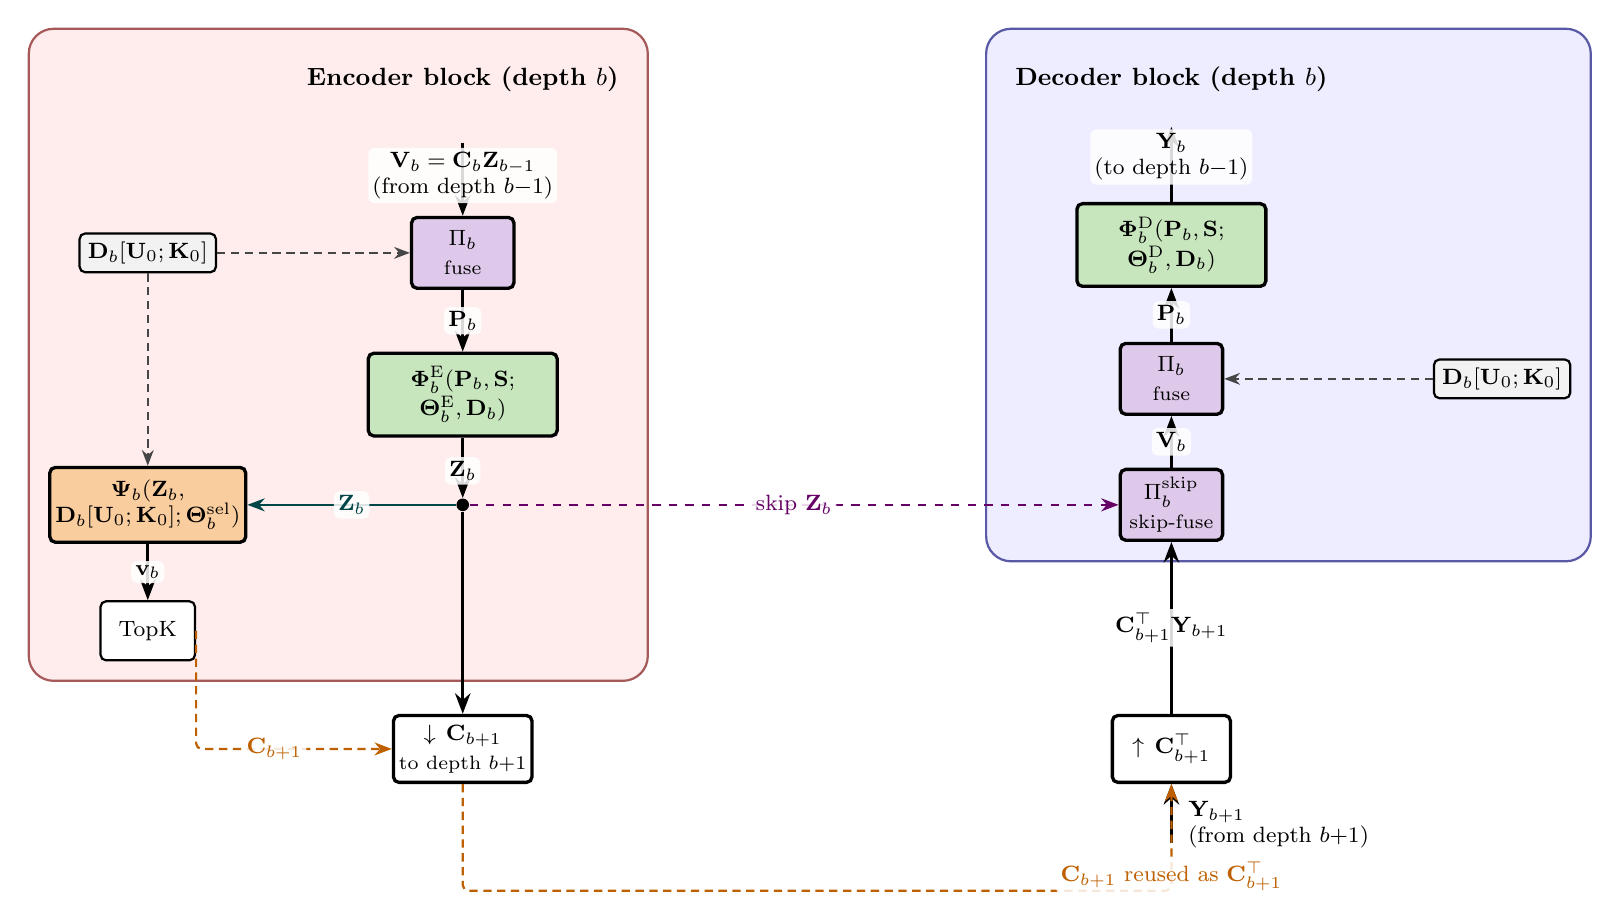
\begin{tikzpicture}[
  >={Stealth[length=2.6mm]},
  rounded corners=2pt,
  proc/.style    = {draw, very thick, rounded corners=2pt, align=center,
                    minimum width=2.4cm, minimum height=1.05cm, inner sep=2pt,
                    font=\footnotesize, fill=gnncol},   % GNN green
  fuseb/.style   = {draw, very thick, rounded corners=2pt, align=center,
                    minimum width=1.3cm, minimum height=0.9cm, inner sep=2pt,
                    font=\footnotesize, fill=projcol},  % projection amber
  encbg/.style   = {rounded corners=9pt, fill=red!7,  draw=red!30!gray, thick,
                    inner sep=7pt},
  decbg/.style   = {rounded corners=9pt, fill=blue!7, draw=blue!30!gray, thick,
                    inner sep=7pt},
  selb/.style    = {draw, very thick, rounded corners=2pt, align=center,
                    minimum width=2.4cm, minimum height=0.95cm, inner sep=2pt,
                    font=\footnotesize, fill=selcol},
  sampb/.style   = {draw, very thick, rounded corners=2pt, align=center,
                    minimum width=1.5cm, minimum height=0.85cm, inner sep=2pt,
                    font=\footnotesize, fill=white},
  condb/.style   = {draw, thick, rounded corners=2pt, align=center,
                    inner sep=3pt, font=\footnotesize, fill=black!5},
  topkb/.style   = {draw, thick, rounded corners=2pt, align=center,
                    minimum width=1.2cm, minimum height=0.75cm, inner sep=2pt,
                    font=\footnotesize, fill=white},
  splitdot/.style= {circle, fill=black, inner sep=0pt, minimum size=1.6mm},
  sig/.style     = {-{Stealth[length=2.6mm]}, very thick},
  feat/.style    = {-{Stealth[length=2.2mm]}, thick, teal!55!black},
  ctrl/.style    = {-{Stealth[length=2.2mm]}, thick, densely dashed, orange!75!black},
  skip/.style    = {-{Stealth[length=2.2mm]}, thick, dashed, violet!80!black},
  condarr/.style = {-{Stealth[length=2.0mm]}, thick, gray!55!black, densely dashed},
  elbl/.style    = {font=\footnotesize, inner sep=1.5pt, fill=white,
                    fill opacity=0.85, text opacity=1},
  hd/.style      = {font=\small\bfseries},
]

% ---------- ENCODER block (depth b) : flows top -> down ----------
\node[fuseb] (Epi)   at (0,6.8) {$\Piblk{b}$\\[1pt]{\scriptsize fuse}};
\node[proc]  (Egnn)  at (0,5.0) {$\PhiEnc{b}(\bbP_b,\bbS;$\\$\thetaenc_b,\bbD_b)$};
\node[splitdot](Esp) at (0,3.6) {};
\node[sampb] (Edown) at (0,0.5) {$\downarrow\,\bbC_{b+1}$\\[1pt]{\scriptsize to depth $b{+}1$}};  % OUTSIDE panel
\node[condb] (Econd) at (-4.0,6.8) {$\bbD_b\UK$};
\node[selb]  (Epsi)  at (-4.0,3.6) {$\Psisel{b}(\bbZ_b,$\\$\bbD_b\UK;\thetasel_{b})$};
\node[topkb] (Etopk) at (-4.0,2.0) {$\mathrm{TopK}$};

\draw[sig]  (0,8.2) -- (Epi.north)
            node[elbl,pos=0.45,align=center]{$\bbV_b=\bbC_b\bbZ_{b-1}$\\(from depth $b{-}1$)};
\draw[condarr] (Econd.east) -- (Epi.west);
\draw[sig]  (Epi.south)  -- (Egnn.north) node[elbl,pos=0.5]{$\bbP_b$};
\draw[sig]  (Egnn.south) -- (Esp)        node[elbl,pos=0.55]{$\bbZ_b$};
\draw[sig]  (Esp) -- (Edown.north);
\draw[feat] (Esp) -- (Epsi.east)         node[elbl,pos=0.5]{$\bbZ_b$};
\draw[condarr] (Econd.south) -- (Epsi.north);
\draw[sig]  (Epsi.south) -- (Etopk.north) node[elbl,pos=0.5]{$\bbvv_{b}$};
\draw[ctrl] (Etopk.east) |- (Edown.west)  node[elbl,pos=0.7]{$\bbC_{b+1}$};

% ---------- DECODER block (depth b) : flows bottom -> up ----------
\node[sampb] (Dup)   at (9,0.5) {$\uparrow\,\bbC_{b+1}^{\top}$};  % OUTSIDE panel
\node[fuseb] (Dskip) at (9,3.6) {$\Piskip{b}$\\[1pt]{\scriptsize skip-fuse}};
\node[fuseb] (Dpi)   at (9,5.2) {$\Piblk{b}$\\[1pt]{\scriptsize fuse}};
\node[proc]  (Dgnn)  at (9,6.9) {$\PhiDec{b}(\bbP_b,\bbS;$\\$\thetadec_b,\bbD_b)$};
\node[condb] (Dcond) at (13.2,5.2) {$\bbD_b\UK$};

\draw[sig]  (9,-0.7) -- (Dup.south)
            node[elbl,pos=0.32,align=left,anchor=west,xshift=4pt]{$\bbY_{b+1}$\\(from depth $b{+}1$)};
\draw[sig]  (Dup.north)   -- (Dskip.south) node[elbl,pos=0.5]{$\bbC_{b+1}^{\top}\bbY_{b+1}$};
\draw[sig]  (Dskip.north) -- (Dpi.south)   node[elbl,pos=0.5]{$\bbV_b$};
\draw[condarr] (Dcond.west) -- (Dpi.east);
\draw[sig]  (Dpi.north)   -- (Dgnn.south)  node[elbl,pos=0.5]{$\bbP_b$};
\draw[sig]  (Dgnn.north)  -- (9,8.4)
            node[elbl,pos=0.6,align=center]{$\bbY_b$\\(to depth $b{-}1$)};

% ---------- cross-links between the two blocks ----------
% skip Z_b : encoder split -> decoder skip-fusion
\draw[skip] (Esp) -- (Dskip.west) node[elbl,pos=0.5]{skip $\bbZ_b$};
% reuse C_{b+1} : encoder selector -> decoder up-sampling
\draw[ctrl] (Edown.south) -- (0,-1.3) -- (9,-1.3) -- (Dup.south)
            node[elbl,pos=0.32,below]{$\bbC_{b+1}$ reused as $\bbC_{b+1}^{\top}$};

% ---------- headers + caption ----------
\node[hd] (Ehdr) at (0,9.0)  {Encoder block (depth $b$)};
\node[hd] (Dhdr) at (9,9.0)  {Decoder block (depth $b$)};

% ---------- half-panel background tints (light red / light blue) ----------
\begin{scope}[on background layer]
  \node[encbg, fit={(Ehdr)(Econd)(Epi)(Egnn)(Esp)(Epsi)(Etopk)(0,9.4)}] {};
  \node[decbg, fit={(Dhdr)(Dskip)(Dpi)(Dgnn)(Dcond)(9,9.4)}] {};
\end{scope}

\ifshowcaption
\node[font=\small, align=center] at (4.5,-2.3)
  {\textbf{Fig.~2.} Block interface. The fusion layer $\Piblk{b}$ is shared across the
   matched encoder/decoder pair; the selection matrix $\bbC_{b+1}$ produced by
   $\Psisel{b}$ on the encoder side is reused (transposed) by the decoder's
   up-sampling. Global embeddings enter as $\bbD_b\UK$.};
\fi

\end{tikzpicture}
}
%       \caption{...}\label{fig:ugnn-block}
%     \end{figure*}
%  NB embedded, fonts inherit YOUR paper's class (not extarticle 17pt);
%  \resizebox scales the whole picture, so it stays internally consistent.
% =====================================================================
\usetikzlibrary{arrows.meta, positioning, calc, backgrounds, fit}

% ===== categorical block palette =====================================
%   green  = GNN  (phi^enc / phi^dec / phi^bn)
%   purple = projection layers (Pi_0, Pi^cond, Pi^step, Pi_b, Pi^skip, Pi_out)
%   orange = learned node selector (Psi_b)  -- matches its C_b control edges
%   red / blue are RESERVED for the encoder / decoder panels.
\definecolor{gnncol}{RGB}{200,230,190}
\definecolor{projcol}{RGB}{223,201,234}
\definecolor{selcol}{RGB}{250,205,158}
\definecolor{bandcol}{RGB}{176,130,80}   % depth-band base (warm golden sand; swap freely)

% ===== math glyphs (\providecommand: figure owns them, but a paper that ====
% ===== already defines the symbol keeps its own version, no clash) ========
\providecommand{\bbS}{\mathbf{S}}
\providecommand{\bbC}{\mathbf{C}}
\providecommand{\bbD}{\mathbf{D}}
\providecommand{\bbZ}{\mathbf{Z}}
\providecommand{\bbY}{\mathbf{Y}}
\providecommand{\bbU}{\mathbf{U}}
\providecommand{\bbK}{\mathbf{K}}
\providecommand{\bbP}{\mathbf{P}}
\providecommand{\bbV}{\mathbf{V}}
\providecommand{\bbI}{\mathbf{I}}
\providecommand{\bbvv}{\mathbf{v}}
\providecommand{\bbx}{\mathbf{x}}
\providecommand{\bbu}{\mathbf{u}}
\providecommand{\bbeps}{\boldsymbol{\epsilon}_{\boldsymbol{\theta}}}
\providecommand{\bbepsilon}{\boldsymbol{\epsilon}}      % bare epsilon (subscript supplied at use site)
\providecommand{\bbtheta}{\boldsymbol{\theta}}
\providecommand{\bbxi}{\boldsymbol{\xi}}                % compact conditioning placeholder (S,u,...)
\providecommand{\alphacumprod}{\bar{\alpha}}            % cumulative-product noise schedule constant
\providecommand{\UK}{[\bbU_0;\bbK_0]}
% GNN operators (single symbol phi, role superscript)
\providecommand{\PhiEnc}[1]{\boldsymbol{\Phi}^{\mathrm{E}}_{#1}}
\providecommand{\PhiDec}[1]{\boldsymbol{\Phi}^{\mathrm{D}}_{#1}}
\providecommand{\PhiBn}{\boldsymbol{\Phi}^{\mathrm{B}}}
% projection / embedding family
\providecommand{\Piin}{\Pi_{0}}
\providecommand{\Picond}{\Pi^{\mathrm{cond}}_{0}}
\providecommand{\Pistep}{\Pi^{\mathrm{step}}_{0}}
\providecommand{\Piblk}[1]{\Pi_{#1}}
\providecommand{\Piskip}[1]{\Pi^{\mathrm{skip}}_{#1}}
\providecommand{\Piout}{\Pi_{\mathrm{out}}}
% scoring head
\providecommand{\Psisel}[1]{\boldsymbol{\Psi}_{#1}}
% learnable parameters
\providecommand{\thetaenc}{\boldsymbol{\Theta}^{\mathrm{E}}}
\providecommand{\thetadec}{\boldsymbol{\Theta}^{\mathrm{D}}}
\providecommand{\thetasel}{\boldsymbol{\Theta}^{\mathrm{sel}}}

% ===== caption toggle (build option) =================================
% Captions ON by default.  Turn OFF either way:
%   * after this \input:  \showcaptionfalse        (e.g. when embedding in a paper)
%   * on the command line: pdflatex "\def\nocaption{}% =====================================================================
%  U-GNN denoiser architecture  (reference: oarfish-9)  --  STANDALONE WRAPPER
%
%  This file is now a THIN WRAPPER, used only for local 2-page preview.
%  The actual drawing code lives in three sibling files:
%      _ugnn_preamble.tex  -- shared colours, glyph macros, caption toggle
%      ugnn_fig1.tex       -- Fig 1 (high-level encoder-decoder U)
%      ugnn_fig2.tex       -- Fig 2 (block-interface inset)
%  To EMBED the figures in a paper, \input the preamble + each body file
%  directly into your main.tex (see the header of _ugnn_preamble.tex for the
%  exact snippet); do NOT \input this wrapper.
%
%  Notation (single GNN symbol phi; conditioning fused by Pi_b before phi):
%    encoder    Z_b   = Phi^E_b ( P_b , S ; Theta^enc_b , D_b )
%    decoder    Y_b   = Phi^D_b ( P_b , S ; Theta^dec_b , D_b )
%    bottleneck Y_{B+1}= Phi^B  ( C_{B+1} Z_B , S ; Theta^bn , D_{B+1} )
%    block fuse P_b   = Pi_b ( V_b , D_b [U_0;K_0] )
%    selection (depth-b selector)  v_b = Psi_b ( Z_b , D_b[U_0;K_0] ) ; C_{b+1} = TopK(v_b)
%
%  Compile (with captions):  pdflatex ugnn_architecture_full.tex
%  Compile (no captions):    pdflatex "\def\nocaption{}\input{ugnn_architecture_full}"
% =====================================================================
\documentclass[tikz,border=12pt,class=extarticle,17pt]{standalone}   % extarticle 17pt base: bigger global fonts
\usepackage{amsmath}
\input{_ugnn_preamble}

\begin{document}
\input{ugnn_fig1}
\newpage
\input{ugnn_fig2}
\end{document}
"
% Guarded so a double \input cannot redefine/reset the flag.
\ifdefined\ifshowcaption\else \newif\ifshowcaption \showcaptiontrue \fi
\ifdefined\nocaption\showcaptionfalse\fi


\begin{document}
\input{ugnn_fig1}
\newpage
% ugnn_fig2.tex -- Fig 2 body (block-interface inset). Drawing only.
% \input AFTER _ugnn_preamble.tex.
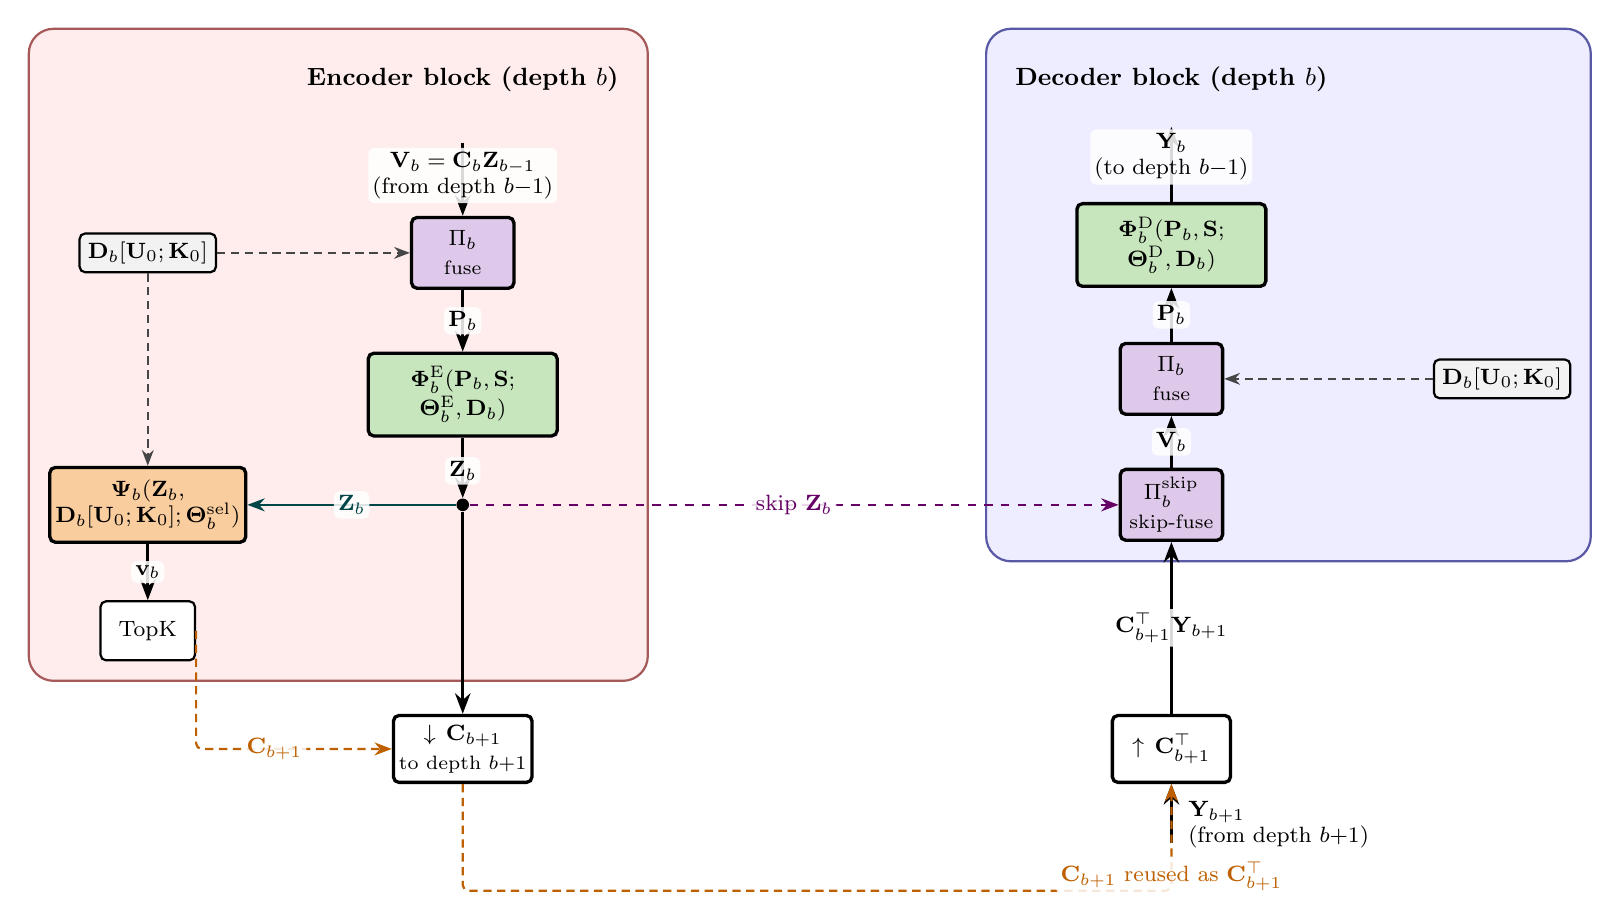
\begin{tikzpicture}[
  >={Stealth[length=2.6mm]},
  rounded corners=2pt,
  proc/.style    = {draw, very thick, rounded corners=2pt, align=center,
                    minimum width=2.4cm, minimum height=1.05cm, inner sep=2pt,
                    font=\footnotesize, fill=gnncol},   % GNN green
  fuseb/.style   = {draw, very thick, rounded corners=2pt, align=center,
                    minimum width=1.3cm, minimum height=0.9cm, inner sep=2pt,
                    font=\footnotesize, fill=projcol},  % projection amber
  encbg/.style   = {rounded corners=9pt, fill=red!7,  draw=red!30!gray, thick,
                    inner sep=7pt},
  decbg/.style   = {rounded corners=9pt, fill=blue!7, draw=blue!30!gray, thick,
                    inner sep=7pt},
  selb/.style    = {draw, very thick, rounded corners=2pt, align=center,
                    minimum width=2.4cm, minimum height=0.95cm, inner sep=2pt,
                    font=\footnotesize, fill=selcol},
  sampb/.style   = {draw, very thick, rounded corners=2pt, align=center,
                    minimum width=1.5cm, minimum height=0.85cm, inner sep=2pt,
                    font=\footnotesize, fill=white},
  condb/.style   = {draw, thick, rounded corners=2pt, align=center,
                    inner sep=3pt, font=\footnotesize, fill=black!5},
  topkb/.style   = {draw, thick, rounded corners=2pt, align=center,
                    minimum width=1.2cm, minimum height=0.75cm, inner sep=2pt,
                    font=\footnotesize, fill=white},
  splitdot/.style= {circle, fill=black, inner sep=0pt, minimum size=1.6mm},
  sig/.style     = {-{Stealth[length=2.6mm]}, very thick},
  feat/.style    = {-{Stealth[length=2.2mm]}, thick, teal!55!black},
  ctrl/.style    = {-{Stealth[length=2.2mm]}, thick, densely dashed, orange!75!black},
  skip/.style    = {-{Stealth[length=2.2mm]}, thick, dashed, violet!80!black},
  condarr/.style = {-{Stealth[length=2.0mm]}, thick, gray!55!black, densely dashed},
  elbl/.style    = {font=\footnotesize, inner sep=1.5pt, fill=white,
                    fill opacity=0.85, text opacity=1},
  hd/.style      = {font=\small\bfseries},
]

% ---------- ENCODER block (depth b) : flows top -> down ----------
\node[fuseb] (Epi)   at (0,6.8) {$\Piblk{b}$\\[1pt]{\scriptsize fuse}};
\node[proc]  (Egnn)  at (0,5.0) {$\PhiEnc{b}(\bbP_b,\bbS;$\\$\thetaenc_b,\bbD_b)$};
\node[splitdot](Esp) at (0,3.6) {};
\node[sampb] (Edown) at (0,0.5) {$\downarrow\,\bbC_{b+1}$\\[1pt]{\scriptsize to depth $b{+}1$}};  % OUTSIDE panel
\node[condb] (Econd) at (-4.0,6.8) {$\bbD_b\UK$};
\node[selb]  (Epsi)  at (-4.0,3.6) {$\Psisel{b}(\bbZ_b,$\\$\bbD_b\UK;\thetasel_{b})$};
\node[topkb] (Etopk) at (-4.0,2.0) {$\mathrm{TopK}$};

\draw[sig]  (0,8.2) -- (Epi.north)
            node[elbl,pos=0.45,align=center]{$\bbV_b=\bbC_b\bbZ_{b-1}$\\(from depth $b{-}1$)};
\draw[condarr] (Econd.east) -- (Epi.west);
\draw[sig]  (Epi.south)  -- (Egnn.north) node[elbl,pos=0.5]{$\bbP_b$};
\draw[sig]  (Egnn.south) -- (Esp)        node[elbl,pos=0.55]{$\bbZ_b$};
\draw[sig]  (Esp) -- (Edown.north);
\draw[feat] (Esp) -- (Epsi.east)         node[elbl,pos=0.5]{$\bbZ_b$};
\draw[condarr] (Econd.south) -- (Epsi.north);
\draw[sig]  (Epsi.south) -- (Etopk.north) node[elbl,pos=0.5]{$\bbvv_{b}$};
\draw[ctrl] (Etopk.east) |- (Edown.west)  node[elbl,pos=0.7]{$\bbC_{b+1}$};

% ---------- DECODER block (depth b) : flows bottom -> up ----------
\node[sampb] (Dup)   at (9,0.5) {$\uparrow\,\bbC_{b+1}^{\top}$};  % OUTSIDE panel
\node[fuseb] (Dskip) at (9,3.6) {$\Piskip{b}$\\[1pt]{\scriptsize skip-fuse}};
\node[fuseb] (Dpi)   at (9,5.2) {$\Piblk{b}$\\[1pt]{\scriptsize fuse}};
\node[proc]  (Dgnn)  at (9,6.9) {$\PhiDec{b}(\bbP_b,\bbS;$\\$\thetadec_b,\bbD_b)$};
\node[condb] (Dcond) at (13.2,5.2) {$\bbD_b\UK$};

\draw[sig]  (9,-0.7) -- (Dup.south)
            node[elbl,pos=0.32,align=left,anchor=west,xshift=4pt]{$\bbY_{b+1}$\\(from depth $b{+}1$)};
\draw[sig]  (Dup.north)   -- (Dskip.south) node[elbl,pos=0.5]{$\bbC_{b+1}^{\top}\bbY_{b+1}$};
\draw[sig]  (Dskip.north) -- (Dpi.south)   node[elbl,pos=0.5]{$\bbV_b$};
\draw[condarr] (Dcond.west) -- (Dpi.east);
\draw[sig]  (Dpi.north)   -- (Dgnn.south)  node[elbl,pos=0.5]{$\bbP_b$};
\draw[sig]  (Dgnn.north)  -- (9,8.4)
            node[elbl,pos=0.6,align=center]{$\bbY_b$\\(to depth $b{-}1$)};

% ---------- cross-links between the two blocks ----------
% skip Z_b : encoder split -> decoder skip-fusion
\draw[skip] (Esp) -- (Dskip.west) node[elbl,pos=0.5]{skip $\bbZ_b$};
% reuse C_{b+1} : encoder selector -> decoder up-sampling
\draw[ctrl] (Edown.south) -- (0,-1.3) -- (9,-1.3) -- (Dup.south)
            node[elbl,pos=0.32,below]{$\bbC_{b+1}$ reused as $\bbC_{b+1}^{\top}$};

% ---------- headers + caption ----------
\node[hd] (Ehdr) at (0,9.0)  {Encoder block (depth $b$)};
\node[hd] (Dhdr) at (9,9.0)  {Decoder block (depth $b$)};

% ---------- half-panel background tints (light red / light blue) ----------
\begin{scope}[on background layer]
  \node[encbg, fit={(Ehdr)(Econd)(Epi)(Egnn)(Esp)(Epsi)(Etopk)(0,9.4)}] {};
  \node[decbg, fit={(Dhdr)(Dskip)(Dpi)(Dgnn)(Dcond)(9,9.4)}] {};
\end{scope}

\ifshowcaption
\node[font=\small, align=center] at (4.5,-2.3)
  {\textbf{Fig.~2.} Block interface. The fusion layer $\Piblk{b}$ is shared across the
   matched encoder/decoder pair; the selection matrix $\bbC_{b+1}$ produced by
   $\Psisel{b}$ on the encoder side is reused (transposed) by the decoder's
   up-sampling. Global embeddings enter as $\bbD_b\UK$.};
\fi

\end{tikzpicture}

\end{document}
"
% Guarded so a double \input cannot redefine/reset the flag.
\ifdefined\ifshowcaption\else \newif\ifshowcaption \showcaptiontrue \fi
\ifdefined\nocaption\showcaptionfalse\fi
